\documentclass[12pt,a4paper,headsepline,footsepline,DIV13,BCOR12mm]{scrbook}
\usepackage[english,ngerman]{babel}
\usepackage[T1]{fontenc}
\usepackage[latin1]{inputenc}
\usepackage{scrpage2}
\pagestyle{scrheadings}

%\usepackage[backend=biber,style=unsrt]{biblatex}

\usepackage{graphicx}

\usepackage{setspace}

\usepackage{tikz}
\usetikzlibrary{arrows, shapes}
\usepackage{amsmath}

% LTL Symbols
\usepackage{latexsym}
\usepackage{MnSymbol}

\usepackage{wrapfig}

\usepackage{listings}
\usepackage{color}
\definecolor{gray}{rgb}{0.4,0.4,0.4}
\definecolor{darkblue}{rgb}{0.0,0.0,0.6}
\definecolor{cyan}{rgb}{0.0,0.6,0.6}

%for bookmark bar
\usepackage[colorlinks,pdfpagelabels,pdfstartview=FitH,bookmarksopen=false,bookmarksnumbered=false,linkcolor=black,plainpages=false,hypertexnames=false,citecolor=black]{hyperref}

\usepackage{algorithm}
\usepackage{algorithmic}



\begin{document}



%PREFACE
\selectlanguage{ngerman}
%%%%%%%%%%%%%%%%%%%%%%%%%%%%%%%%%%%%%%%%%%%%%%%%%%%%%%%%%%%%%%%%%%%%%%%%%%%%%%%%%%%%
%%% Title-Page
\thispagestyle{empty}

\begin{table}[h]
\centering
\begin{tabular}{ccc}

\includegraphics[width=.18\linewidth]{img/logos/lmu_logo} \hspace{0.7cm} &

\includegraphics[scale=0.18]{img/logos/Uni_Aug_Logo_Basis_pos_A}
\hspace{0.7cm} &

\includegraphics[scale=0.86]{img/logos/tum}
\end{tabular}
\end{table}

\vspace{8mm}
\begin{center}
{\Large
{\bfseries \scshape Institut f�r Software \& Systems Engineering}\\
Universit�tsstra�e 6a \hspace{0.25cm} D-86135 Augsburg\\
}
\end{center}

\vspace{1cm}
%title
\begin{center}
{\Huge \bfseries Graphical formalization and \\
\vspace{0.25cm}
automated computing of safety \\
\vspace{0.25cm}
constraints in robotics 
}
\end{center}

\vspace{1.5cm}
%author
\begin{center}
{\Large Ludwig N�gele}
\end{center}

\vspace{1cm}
\begin{center}
{\Large \bfseries Masterarbeit im Elitestudiengang Software Engineering}
\end{center}

\vspace{1cm}
\begin{center}

\includegraphics[width=.4\linewidth]{img/logos/LogoSEengl}
\end{center}



%%%%%%%%%%%%%%%%%%%%%%%%%%%%%%%%%%%%%%%%%%%%%%%%%%%%%%%%%%%%%%%%%%%%%%%%%%%%%%%%%%%%
%%% Advisor-Page
%%%%%%%%%%%%%%%%%%%%%%%%%%%%%%%%%%%%%%%%%%%%%%%%%%%%%%%%%%%%%%%%%%%%%%%%%%%%%%%%%%%%
\newpage
\thispagestyle{empty}
\mbox{}
\newpage
\thispagestyle{empty}

\begin{table}[h]
\centering
\begin{tabular}{ccc}

\includegraphics[width=.18\linewidth]{img/logos/lmu_logo} \hspace{0.7cm} &

\includegraphics[scale=0.18]{img/logos/Uni_Aug_Logo_Basis_pos_A}
\hspace{0.7cm} &

\includegraphics[scale=0.86]{img/logos/tum}
\end{tabular}
\end{table}

\vspace{8mm}
\begin{center}
{\Large
{\bfseries \scshape Institut f�r Software \& Systems Engineering}\\
Universit�tsstra�e 6a \hspace{0.25cm} D-86135 Augsburg\\
}
\end{center}

\vspace{0.6cm}
%title
\begin{center}
{\Huge \bfseries Graphical formalization and \\
\vspace{0.25cm}
automated computing of safety \\
\vspace{0.25cm}
constraints in robotics
}
\end{center}

\vspace{0.8cm}
%author
\begin{center}
\begin{table}[h]
\centering
\begin{tabular}{ll}
Matrikelnummer: & 1168616 \\
Beginn der Arbeit: & 06.\ Juni 2012 \\ 
Abgabe der Arbeit: & 16.\ November 2012 \\
Erstgutachter: & Prof.\ Dr.\ Wolfgang Reif \\
Zweitgutachter: & Prof.\ Dr.\ Bernhard Bauer \\
Betreuer: & M.Sc. Andreas Angerer \\
\end{tabular}
\end{table}
\end{center}

\vspace{0.8cm}
\begin{center}

\includegraphics[width=.4\linewidth]{img/logos/LogoSEengl}
\end{center}

%%%%%%%%%%%%%%%%%%%%%%%%%%%%%%%%%%%%%%%%%%%%%%%%%%%%%%%%%%%%%%%%%%%%%%%%%%%%%%%%%%%%
%%% Statement-Page
\newpage
\thispagestyle{empty}
\mbox{}
 




\onehalfspacing
\newpage
\thispagestyle{empty}

\centerline{\bfseries ERKL�RUNG}

\vspace{5cm}
Hiermit versichere ich, dass ich diese Masterarbeit selbst�ndig verfasst habe.
Ich habe dazu keine anderen als die angegebenen Quellen und Hilfsmittel
verwendet.

\vspace{1cm}
\begin{flushleft}
%select german for formatting the date
\selectlanguage{ngerman}
Augsburg, den \today \hfill Ludwig N�gele
\end{flushleft}

\newpage
\thispagestyle{empty}
\mbox{}







\newpage


%select english as language!
\selectlanguage{english}
%\pagenumbering{roman}
\pagenumbering{arabic}

\pdfbookmark[1]{Inhaltsverzeichnis}{toc}
\tableofcontents
\newpage
\listoffigures
\newpage
%\listoftables
\lstlistoflistings
%\pagenumbering{arabic}

\graphicspath{{./images/}}
\DeclareGraphicsExtensions{.jpg}


\chapter*{Abstract}

Nowadays robotic applications are no longer confined to only industrial use but increasingly assigned to jobs within human workspaces. Even the programming of robots is shifting from experienced software developers to the consumers themselves who need to customize the robot's behavior in order to match individual requirements.
However both the human robot collaboration as well as the behavior definition by non experts may be a risk to humans within the robots' environment.
Thus special thinking is needed about how to cope with safety requirements for robot behavior specification by consumers.

In this paper we present a visual language for the defining of safety constraints for state machine definition of robot behaviour. Our approach addresses mainly non-safety-experts and our abstraction from a mathematical temporal logic expression to a more intuitive visual representation is intended to enable a wider range of software developers to do model checking.
Furthermore we propose a new concept of development support by providing automated constraint generation functionality. It aims to help developers in defining reasonable constraints and finally to increase the probability of finding bugs.

A graphical editor has been developed which demonstrates both visual constraint creation functionality as well as automated constraint generation.
\chapter{Introduction}

Safety critical robot applications require extensive testing or formal verification in order to achieve adequate safe and predictable behaviour.
Even if a program does not control actuators itself and thus cannot directly cause any damage, its output might still be a trigger for dangerous actions involving several actors.
Imagine a medication reminder application running on a service robot which guides a person through the process of medication intake, as investigated in the healthcare robotics project at the
\begin{wrapfigure}{r}{0.58\textwidth}
  \centering
  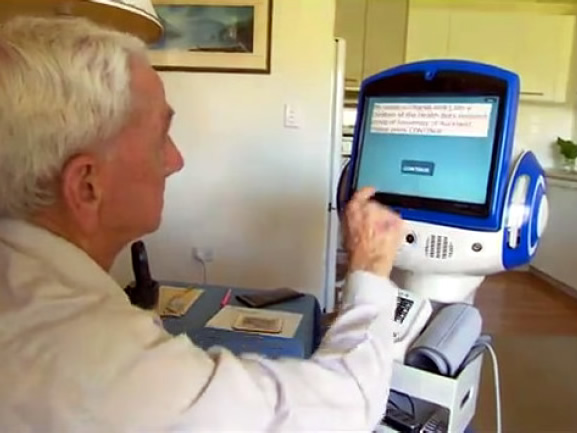
\includegraphics[width=0.56\textwidth]{cafero_being_used}
  \caption{Service robot being used by older person~\cite{robostudio}.}
  \label{fig:cafero_being_used}
\end{wrapfigure}
Uni\-ver\-si\-ty of Auckland, New Zealand \cite{jayawardena12:_desig}. All interaction is gui\-ded by showing textual instructions on a display, and by speech generation. An error in the program logic could cause an already taken medication to be reminded again and may injure a patient with Alzheimer's disease by causing a medication overdose.
Scientists are working on applications such as the medication reminder~\cite{p11:_feasib} which run on mobile robots (so called healthbots) serving in nursing homes for the elderly. Equipped with a touch display and several external devices such as a blood pressure measurement tool the robots aim to support and entertain the elderly in their daily activities~\cite{jayawardena12:_desig,5649910}.

With service robots coexisting with people and acting within their work\-spa\-ces, coping with reliability and safety issues is essential for trust and acceptance of these robots. In some cases safety certifications based on international standards for functional safety might be even required before robots get released for use or obtain concession for sale. One such international standard is IEC 61508~\cite{iec61508}, a basic functional safety standard targeting all kinds of industry.
ISO 13482~\cite{iso13482, iso13482-2} is still under development and is intended to be a harmonised European standard for safety requirements for robots in personal care applications.
However, considering functional safety while developing service robots is both complex and difficult; maybe one reason for the absense of safety checks and assurances in the current healthbot versions at the University of Auckland.
But facing the fact that safety requirements for service robots are expected to increase in future, there is a plan of slowly integrating safety functionality into the healthcare robotics project as a next step starting with the concepts introduced in this paper.

The applications for the healthcare robots mentioned above are intended to be developed by healthcare professionals using Robostudio~\cite{robostudio}, a visual programming environment for rapid authoring and customization of complex robot services.
%state machine based processes and a graphical tool for the designing of human robot interaction.
Generally these people do not have profound knowledge of the complex mathematical syntax used for formal methods which allow software behaviour verification.
%temporal logic such as computation tree logic (CTL) or linear temporal logic (LTL).
Nevertheless, certain safety guarantees must somehow be delivered in order to gain users' trust and to prevent any harm or injuries by the healthcare robots.
In case of the medication reminder mentioned above it might be important to ensure that notifications are sent to staff members whenever medication is not taken by the patient, or to avoid duplicate reminders for medication which has already been taken.
A mechanism like this is needed for the specification of such safety constraints; one that does not require special or expert knowledge and is thus easy to use for all kind of programmers. Within the scope of this work a visual language has been developed intending to fill this gap.

Unfortunately, supplying an easy-to-use editor for constraint creation does not guarantee adequate thinking about sufficent constraints by the developer. Unmotivated or just unexperienced developers may miss important constraints needed in order to achieve a certain safety level.
To support the user in finding significant constraints it might be useful to automatically compute constraint suggestions which make true testimonies about the current designed program. First of all the generated constraints provide an opportunity for the developer to identify reasonable constraints as well as contradictions between constraints and specification. The latter would mean there are errors in the program which lead to undesired constraints. Furthermore, once constraints are created and checked for sanity they can be validated after every program change and thus ensure integrity during the entire development process. This work introduces a new heuristics for finding such reasonable safety constraints based on state machine definitions that describe robots' behaviours.

Both ideas, the viual language and the automated constraint generation, have been developed and integrated by the author into Robostudio in order to simplify respectively facilitate the use of safety mechanisms for application development for service robots. Thereby the desired safety certification for the healthcare service robots can move closer by one step.

This work starts with background information about the healthcare domain, short explanations of common safety mechanisms and insights into related work in chapter~\ref{chap:background}. After the goals have been described in chapter~\ref{chap:goals}, the visual formalisms and the automated constraint generation are introduced in chapters~\ref{chap:visualformalismsforsafetyconstraints} and~\ref{chap:automatedgenerationofsafetyconstraints}.
A prototype implementation is demonstrated in chapter~\ref{chap:theltlcreatorprototype}, and a test scenario is described in chapter~\ref{chap:testscenarioandevaluation} where the presented tools get evaluated.
Chapter~\ref{chap:conclusionandfuturework} gives a short conclusion and an outlook how the presented work could be continued.

%Once such constraints are defined, they determine the grade of safety coverage. Unfortunately, the program may still contain errors if there is at least one significant constraint missed out. To support the user in finding such ones the tool could furthermore automatically compute suggestions for possible constraints based on the designed statemachine. These are displayed to the programmer and may help him identifying reasonable constraints as well as contradictions between program and specification.

%Our approach presented in this paper has a special focus on the healtcare domain.


%Dieses beispiel ist eine Anwendung eines umfangreichen Healthcare-Projekts, an dem im robotics lab der Universit�t von Auckland gearbeitet wird. Die zustansbasierten Anwendungen laufen auf Cafero, einem mit blutdruckmessger�t und anderen tools austestatteten mobilen Roboter mit Touchdisplay.
%Die einzelnen Anwendungen werden von Healthcare-Professionals mit dem Tool Robostudio [cite] entwickelt, das eine graphische oberfl�sche zur modellierung von zustandsmaschinen externen services und  bietet.
%Allerdings haben diese not to have profound knowledge of the complex mathematical syntax used for formal verification methods such as computation tree logic (CTL) or linear temporal logic (LTL)).
%Dennoch m�chte man gegen�ber den Patienten, die von solchen Robotern gepflegt werden, ein gewisses Level an Sicherheit gew�hrleisten k�nnen. Beispielsweise soll in obigem Beispiel sichergestellt werden k�nnen, dass ein Medikament nach der Einnahme nicht erneut in einer Erinnerung auftaucht, oder dass bei Nichteinnahme ein Mitarbeiter benachrichtigt wird.
%Dazu bedarf es allerdings Mechanismen zur spezifizierung solcher Sicherheitseigenschaften, die f�r den Programmentwickler zug�nglich und einfach (am besten ohne spezialwissen) zu benutzen sind.


%Among others robots are alredy used in elderly care centers for healthcare purpose.

% -->

%Robostudio (oder healthcare applikation) soll irgendwann Sicherheitszertifizierung bekommen (erklaeren warum). Daher ist es wichtig, sicherheitsmechanismen zur verfuegung zu stellen. Einen kleinen Schritt in diese Richtung m�chten wir mit dieser Arbeit machen...
%Anwender kommen aus verschiedenen Domaenen => need of easy-to-use safety functionality


%Aiming for safe and reliable robots,
%IEC 61508 certification. It contributes to reducing costs and development time when creating highly-dependable and safe robots.



%Glossary IEC 61508
%IEC 61508 is an international standard, produced in 2000 by the IEC, for the realisation of functional safety in devices utilising computer technology. Functional safety differs from inherent safety in that its goal is to reduce risk to permissible levels using active techniques, rather than passive techniques. IEC 61508 specifies guidelines for developing safety-related hardware and software, and management techniques for development processes to ensure accurate designs and implementations.
% <--
\chapter{Background}
\label{chap:background}

The subject of this work evolved from the situation, that the healthcare robotic applications of the University of Auckland should be equipped with mechanisms for ensuring safety.
The motivation for it is described in section~\ref{sec:healthbotapplication} as well as the robots, the kind of applications running on them, and their technical background.

The visual programming environment used for the programming of these robots is presented in section~\ref{sec:robostudio}.
For the understanding of safety concepts which this work is based on, a short introduction into the world of functional safety is given in section~\ref{sec:behaviourchecking}. In section~\ref{sec:relatedwork} other works and programs related to this work's topic are examined which also deal with safety aspects.




\section{Healhbot application}
\label{sec:healthbotapplication}

%\begin{wrapfigure}{r}{0.38\textwidth}
%  \centering
%  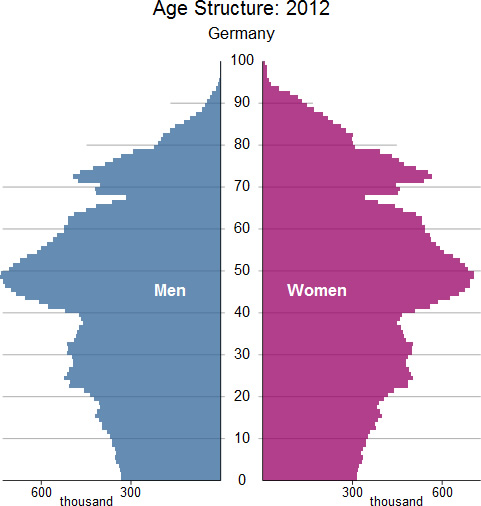
\includegraphics[width=0.34\textwidth]{populationpyramide}
%  \caption{Age structure.}%Population pyramide of germany.}
%  \label{fig:populationpyramide}
%\end{wrapfigure}
In some countries, among New Zealand and Germany, the average age of population is constantly increasing. Owing to excellent achievements in medicine as well as higher living standards, humans can enjoy longer lifes. Also decreasing birth rates contribute to an upward drift of the dominating age range. As a result, the industrial sectors of professional health care and social institutions are required more than ever.
However, a strong deficit of professionals is denoted in the healthcare branch and availability is far behind demand. One reason for this might be below average low salaries for employees in the healthcare sector. But, just raising the salary isn't leading to the desired results since the majority of the older people can't even afford a nurse to today's prices.

Aiming for fillig the constantly increasing gap in professional personnel for healtcare of the elderly and bypassing die financial burden, service robots are supposed to more and more undertake the task of care.
There are lots of possible tasks a robot could do such as taking the blood pressure, guiding medication intake, detecting falls or just entertaining with music, video or internet.
This challenge as a goal, the healtcare robotics team at the University of Auckland researches this topic and builds service robots for supporting the elderlies in their daily life.

The two newest robots IrobiQ and Cafero are shown in figure~\ref{fig:irobiq_cafero}.
These mobile 
\begin{wrapfigure}{r}{0.60\textwidth}
  \centering
  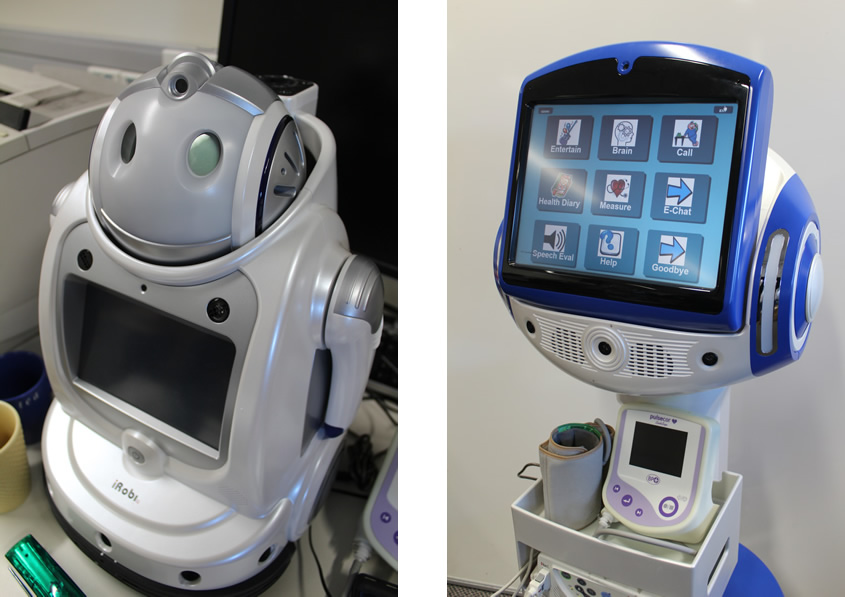
\includegraphics[width=0.56\textwidth]{irobiq_cafero}
  \caption{IrobiQ and Cafero, two robots of the healtcare project.}
  \label{fig:irobiq_cafero}
\end{wrapfigure}
robots have got a touch display for presenting screens and receiving user input. Furthermore they are equipped with additional external tools such as the blood pressure measurement device.
Applications running on the robot use the touch display to present screen dialogs to the user and use speech synthesis in order to give also accoustic feedbak. User inputs or response from devices cause dialogs to change. Figure~\ref{fig:screenflow_example} presents a little example of such a screen-flow based application, which uses response from a camera and user input for navigating through the screen-flow.

%, and they can access devices such as the camera for face recognition or the blood pressure measurement tool. 

There is a program interpreter running on the robots which can load and execute program files. Screen dialogs get generated and displayed on the touch screen.
%This makes the program behaviour replaceable and maintenance can be done easily.
The interpreter processes programs written in Robot Behaviour Description Language (RBDL), a particular DSL based on XML, which has been developed particularly for the healthcare robotic applications. It allows defining state machine based program behaviour and creating UI elements for screen visualizations. An example implementation of one state in RBDL is shown in listing~\ref{lst:RBDL}.

\begin{figure}[htbp]
  \centering
  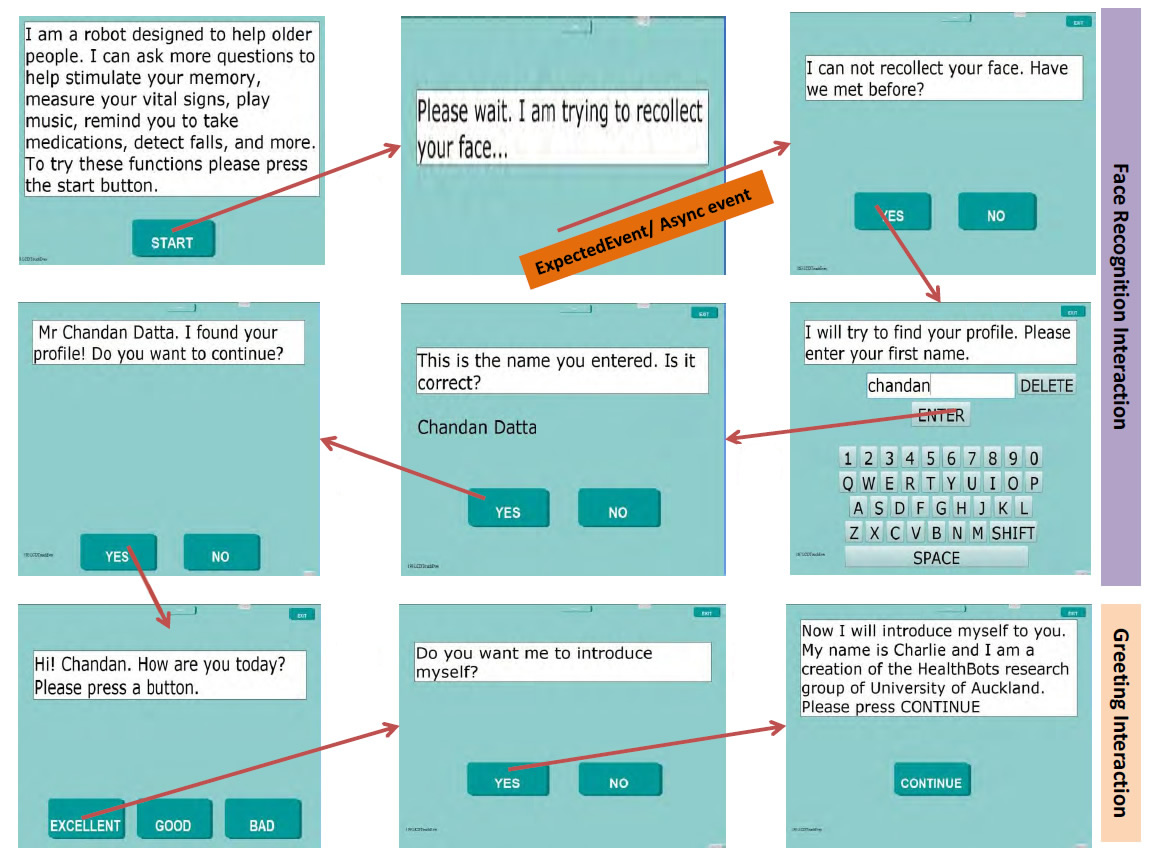
\includegraphics[width=\linewidth]{screenflow_example} 
  \caption{Robot screen-flow dialog based interaction example~\cite{robostudio}.}
  \label{fig:screenflow_example}
\end{figure}

\lstset{
  basicstyle=\ttfamily,
  columns=fullflexible,
  showstringspaces=false,
  commentstyle=\color{gray}\upshape
}

\lstdefinelanguage{XML}
{
  morestring=[b]",
  morestring=[s]{>}{<},
  morecomment=[s]{<?}{?>},
  stringstyle=\color{black},
  identifierstyle=\color{darkblue},
  keywordstyle=\color{cyan},
	morekeywords={%no, type_, senderid, receiverid, name_, vartype, label, width, height, x, y, textsize, preconditions
	}
}

\begin{lstlisting}[float = htbp, language=XML, captionpos=b, breaklines=true, showspaces=false, showtabs=false, tabsize=2, caption=Example of a state defined by RBDL~\cite{robostudio}., label=lst:RBDL]
<state no="84">
	<backgroundactions>
		<rocosmessage type="EVENT MESSAGE" senderid="RCP" receiverid="NA" name="FDSessionStart">
			<parameter vartype="text" type="unsigned int" name="id">1</parameter>
			<parameter type="string" name="" />
		</rocosmessage>
	</backgroundactions>
	<screen>
		<components>
			<button label="START" width="250" height="100" x="387" y="600" textsize="40">
				<event name="clicked">
					<action preconditions="no" name="transition">
						<parameter>
							<type>state</type>
							<name>n</name>
							<value>86</value>
						</parameter>
					</action>
				</event>
			</button>
		</components>
	</screen>
	<expectedevents>
		<event name="TimeOut">
			<action preconditions="no" name="transition">
				<parameter>
					<type>state</type>
					<name>n</name>
					<value>VARFirstScreen</value>
				</parameter>
			</action>
		</event>
	</expectedevents>
</state>
\end{lstlisting}

For each state of the program, backgroundactions can be defined. They are transparent to the user and run in background. Text messages can be sent or external devices can be acessed, for example. The latter is realized with web services to obtain a modular design.
Some states can also have screen definitions with buttons, messages, videos, etc. on it. These are displayed to the user when the particular state is active. Once displayed, buttons can be clicked and trigger events.
The behaviour of events can be mapped in the expectedevents tag. It lists all events which are processable by the current state and defines the correspondend behaviour such as triggering transitions to other states.

For this work the most important thing about the RBDL to remember is, that it can define state machine behaviour with states, transitions and events. This fact was basement for later decisions regarding used safety mechanisms.



%Zugriff auf devices via web services
%Windows is used as operating system on the robots and the programs are executed in Adobe flash and Actionscript. External devices are accessed over web




\section{Robostudio}
\label{sec:robostudio}

In the beginning all programming of the robot behaviour was done by directly editing the XML code mentioned in the previous section by using a text editor. But huge code files and occasional code edits made further maintenance and change requests difficult up to impossible to realise. For this reason Chandan Datta, PhD student at the University of Auckland, developed a visual programming environment for developing robot behaviour on top of RBDL: Robostudio~\cite{robostudio} allows to easily edit the program behaviour on a visual layer and generates the corresponding program file containing the RBDL code fully automatically. This file can be downloaded to the robot and executed by the interpreter. Figure~\ref{fig:robostudio_proceeding} illustrates what the steps of robot behaviour development are.

\begin{figure}[htbp]
  \centering
  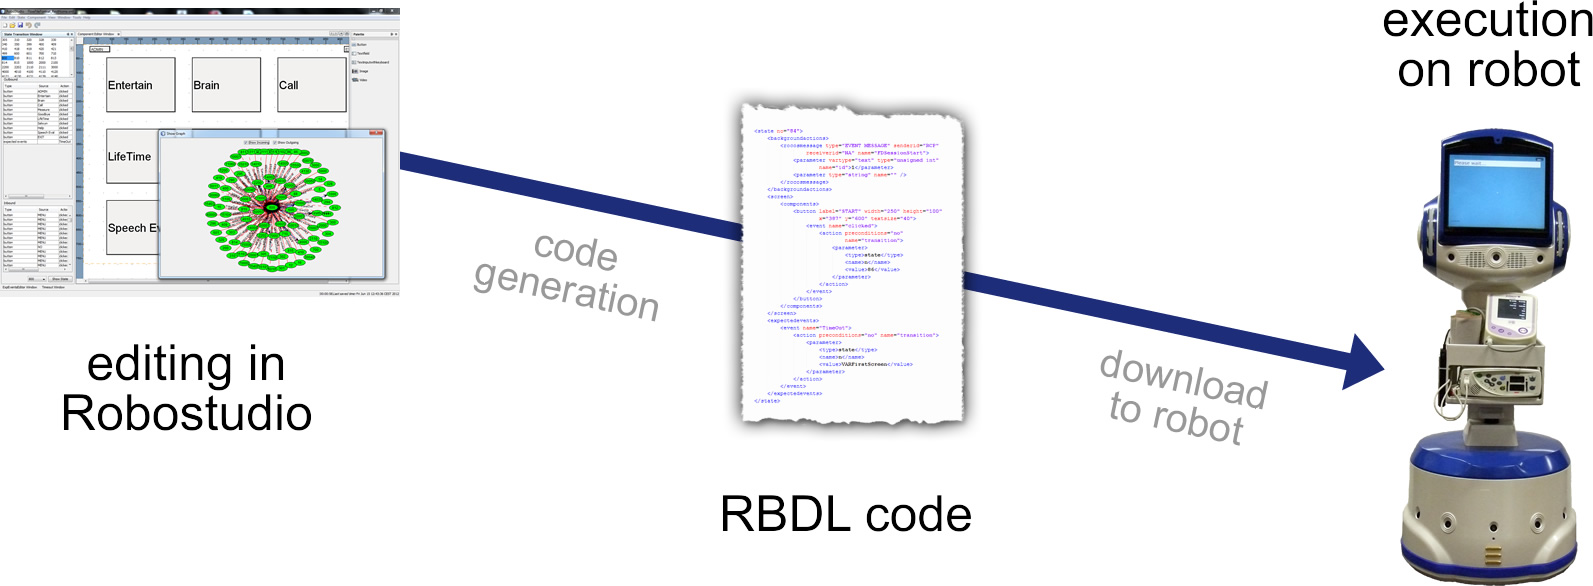
\includegraphics[width=\linewidth]{robostudio_proceeding} 
  \caption{How Robostudio is used for robot behaviour development.}
  \label{fig:robostudio_proceeding}
\end{figure}

Robostudio is an editor fully written in Java and implemented as a NetBeans rich client application.
In several windows and views there are visual tools for editing and understanding robot behaviour as well as screen dialog design. As depicted in figure~\ref{fig:robostudio_vpe} the editor has got a State Navigator Window (1) in the top left corner where all existing states are listed. Underneath an overview about all incoming and outgoing transitions is given. New states can be created and existing states can be deleted. A click on one particular state id in the State Navigator Window will cause all other components to show all possible information regarding to the selected state.
The Expected Events Editor Window (2) in the bottom left provides specifying the expected events and their effects.
Heart and center of the editor is the UI Component Layout Editor Window (3). It renders the screen dialog of the selected state and gives a preview of the screen presented on the robot during runtime. Components such as buttons, text boxes or images can be added, changed or removed via drag and drop.
They are provided by the UI Components Palette Window (4) on the right side where the user can choose from all supported UI components.
The Background Actions Editor Window (5) lets the user define background actions, which are executed trasparently to the user such as accessing external devices or sending messages.
Aiming for supporting the developer with helpful graphical tools the State Transition Visualization Window (6) gives an overview about all connections towards and from the selected state. It helps to quickly get an understanding of the local program behaviour.

\begin{figure}[htbp]
  \centering
  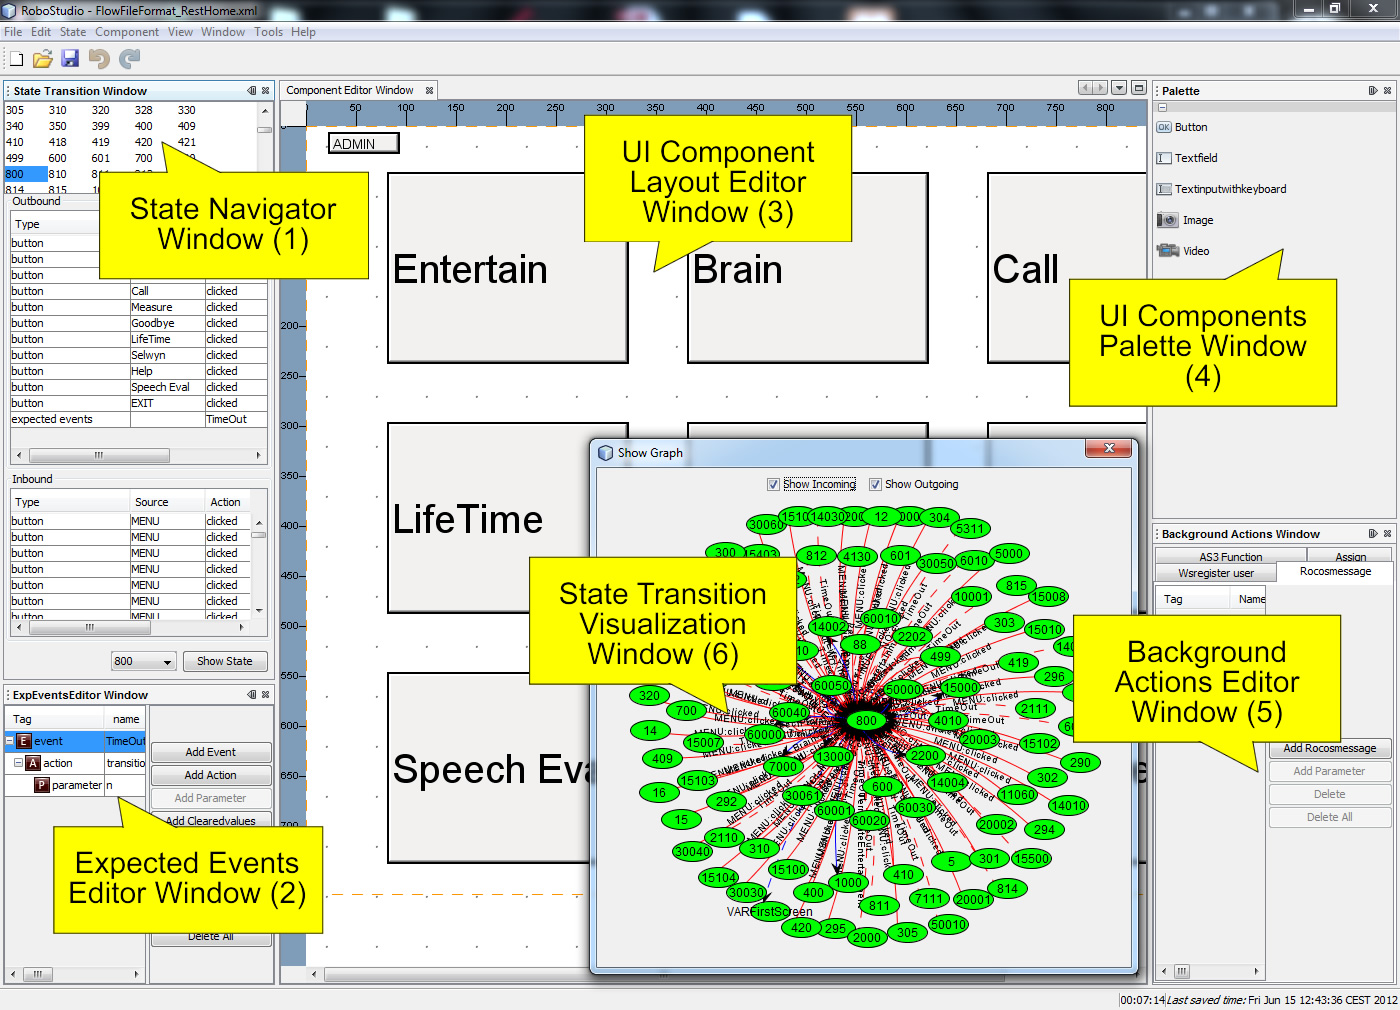
\includegraphics[width=\linewidth]{robostudio_vpe} 
  \caption{Window composition in Robostudio.}
  \label{fig:robostudio_vpe}
\end{figure}


%TODO: Vlt herausstellen, dass eine Schwierigkeit darin bestand, Verhaltensmodellierung und graphische Gestaltung unter einen Hut zu bringen (dazu Bild aus datta paper?). One challenge...






\section{Behaviour checking}
\label{sec:behaviourchecking}

The use of software is versatile from text editing programs running on personal computers, over control software for high-precision applications in aeronautics, right up to trigger mechanisms for deathly weapons. For most of them safety properties are irrelevant, but a few are ranked highly dangerous to their environment and also human lifes. In order to eliminate software malfunction there are a lot of mathematical concepts for verifying software behaviour.
One of them is model checking wich allows checking for functional safety on state machine programs. Since we deal with state machines in the healthbot applications mentioned in section~\ref{sec:healthbotapplication}, this concept of behaviour checking is applicable and important for our kind of programs. At first the basic idea of state machines is described in section~\ref{sec:statemachines}, followed by an intorduction into model checking in section~\ref{sec:modelcheckingandltl}.


\subsection{State machines}
\label{sec:statemachines}



\subsection{Model checking \& LTL}
\label{sec:modelcheckingandltl}

%CTL and LTL are important concepts for model checking and verification of statemachines. But their powerfulness is reflected in the complexity of their mathematical expressions, what makes it difficult to use for programmers who haven't got deeper expertise in this subject.


%NuSMV erwaehnen, erklaeren warum nicht CTL? ltl passt fuer healthcare besser






\section{Related work}
\label{sec:relatedwork}


%Was gibt es schon alles?

% 1993 A Visual-Programming Environment for a Temporal Logic Language
% 1995 Visual Specification of Branching Time Temporal Logic
% 2007 HomeTL: A visual formalism, based on temporal logic, for the design of home based care
% 2007 A Visual Editor to Support the Use of Temporal Logic for ADL Monitoring


A first step towards a graphical tool for designing safety constraints is taken by Sisiruca and Ionescu~\cite{332301}. They developed an object-oriented graphical environment for visually creating temporal logic sentences and rules. The tool presents temporal operators as logical modules with boolean inputs and outputs which can be connected to one big expression graph. Del Bimbo et al. worked on a visual tool for temporal logic, but with a special focus on hierarchical representation of formulas~\cite{520786}. Here each node of a tree is described by an abstract operator whose subformulas are branches to their replacement operators. Thus the root node represents the entire formula. They also explored the formula trees' 3D representation within a virtual space. Both approaches are different fundamental ideas of representing temporal formulas. Whereas having a graph  seems not to be applicable for our approach, the idea of hirarchical operator representation of Del Bimbo et al. will be a good basis for our concept of constraint creation and understanding.

%aim for simplifying the development of constraints, but they still demand knowledge of the underlying mathematical formalism of temporal logic.

The step towards a more abstract level of development is taken by HomeTL~\cite{4341725}, a visual formalism for the design of home based care. It allows healthcare professionals to specify rules and sequences of user actions in a quite nontechnical manner. Based on these conditions a monitoring system in a patient's home environment can detect and report abnormal situations within the daily routine. Even though this approach touches the subject of healthcare it barely matches our problem. HomeTL focuses more on monitoring temporal boundaries of a patient's behaviour than on ensuring functional safety of an implemented program. It does depict how nontechnical constraint design can be realised and its graphical design is a good example of handling time dependencies.

%There are already works about constraint generation such as one approach of NASA [4], for example. They used test oracles in order to achieve consistency between program code and specification during development. 
% Das wollen wir auch erzielen mit unseren automatisch generierten constraints...

%But these kind of oracles are for automated test purpose and are rather complex than intuitive. However, our goal is to find nonmathematical and just intuitive ones. An intelligent heuristic must determine key states and possible conjunctions of them in order to build reasonable constraints. Afterwards they get filtered by an algorithm which computes importances for each constraint based on state weights. Finally the developer obtains a set of visual constraints which he can then check for plausibility.





\subsection{Sisiruca and Ionescu}
\subsection{Del Bimbo (3D)}
\subsection{HomeTL}
\chapter{Goals}
\label{chap:goals}

% soll hier noch gesagt werden, dass wir davon ausgehen, dass es keine endzust�nde gibt?

Ausgehend vom Ziel, die healthcare applikationen des healthcare projects der Universit�t Auckland gewissen Sicherheitsstandards n�her zu bringen und somit einen Schritt in Richtung Sicherheitszertifizierung zu machen, sollen dem VPE Robostudio hierf�r notwendige Werkzeuge hinzugef�gt werden. Dieses Tool(VPE) wird zur Entwicklung von Roboterapplikationen in Form von Zustandsmaschinen verwendet und soll zuk�nftig eine neue Schnittstelle bieten, �ber die der Programmierer das Roboterverhalten auf funktinale Sicherheit hin �berpr�fen kann. Diese Erweiterung soll zum einen nahtlos in Robostudio integriert sein, zum anderen soll es so umgesetzt sein, dass es �ber eine �bersichtliche API auch in andere Programme einfach eingebunden werden kann.

We want to introduce a visual language for defining safety constraints in state machine definitions of robot behaviour, that is suitable for people who are not experts in formal methods. The visual language should be easy to use and intuitive to read, in order to facilitate maintainability.
Hence, the graphical formalism should abstract from the usually complex and mathematical concept of conventional temporal logic but still be significantly expressive.
 
Furthermore we want to integrate some mechanism to support users in finding suitable constraints for a certain application. We assume that applications are modeled by state transition graphs. This modeling paradigm is used in many healthcare robots that employ dialogue systems for communicating with users~\cite{Bickmore2006}. Other possible fields might be shop assistant robots or entertainment robots. For such systems, our approach is suitable. It is based on heuristically analyzing state transition graphs and deriving constraints related to the graph structure. In this work, we want to investigate a particular heuristic as a first step towards user support. 

Finally, we will present some results of applying this heuristics to the medication reminder example described before. The minimum goal that should be achieved was the identification of the following constraints:

\begin{itemize}
	\item The application will always eventually check the database for new reminder jobs. Thus we ensure that pending reminders are processed.
%	\item Either a reminded medication is taken properly, or caregivers are notified that the patient refused medication intake.
	\item Whenever there is a pending reminder, medication will be finally taken or caregivers will get notified in case of the patient refusing medication intake.
% The next item is left out so that we can say, our heuristic found one we didn't think about yet :)
%	\item During the medication intake process the program can not switch to other services such as entertainment mode ore blood pressure measurement, for example.
\end{itemize}

Some of the statements do not make sense if patients lie or pretend to take their medication but don't take it. As our approach validates state machine behaviour rather than human attitudes we assume there is either cooperation from the patient or a separate tool that can verify medication intake. Furthermore we assume the correctness of external services used by the medication reminder such as the database module holding all reminders.

% Bruce: I'm not sure we need this sentence. I think you have integrated it now anyway.
% All the functionality mentioned above shall be combined in one editor and for evaluation purpose later be integrated into a programming environment for state machine editing.
%\chapter{Design}
%\label{chap:design}
%
%
%In this chapter we introduce a first approach of a visual formalism and later state the final desing of the visual language. Furthermore the idea of automated constraint generation is presented in section~\ref{sec:automatedconstraintgeneration}. The assembly of all the previous features in one tool is described in section~\ref{sec:coalescence}. However, the tool's functionality shall also be available in Robostudio in order to provide safety mechanisms for the healthcare service robots. Section~\ref{sec:integrationintorobostudio} gives a main idea how an integration into Robostudio ought to be. 
%
%%The challenge now is to find a similar intuitive and nonmathematical way of representing reasonable safety constraints for the healthbot domain and to figure out how to translate it to corresponding textual expressions. The new concept will be integrated into Robostudio, a design tool for statemachines, in order to enable the user to create safety constraints visually. A common LTL model checker will be added to it as well which fulfils the verification of the translated constraints on the designed statemachine. In case of verification failures the concerning constraints and a visual counter example can be presented.




\chapter{Visual formalisms for safety constraints}
\label{chap:visualformalismsforsafetyconstraints}

This chapter introduces two different approaches of visual formalisms and later states the final desing of the visual language.
One main difficulty in finding a proper visual formalism is to glean the right level between abstraction and expressiveness since this two characteristics appear to be mutually exclusive in some points. A first approach, so called template constraints,
% and its pros and cons 
are described in section~\ref{sec:templateconstraintformalism}. Subsequently a different design - the operator constraint formalism - is presented in section~\ref{sec:operatorconstraintformalism}.
Section~\ref{sec:comparison} gives a comparison of the two formalisms presented before and states which one is used for the prototype.




\section{Template constraint formalism}
\label{sec:templateconstraintformalism}

%It is not a trivial issue to find a
What visual presentation of constraints would suit a healthbot application developer and what are the main types of safety constraints he could want to check?
% TODO: wir haben gedacht, dass es einfach zu benutzen ist
Led by this question, a visual language based on templates has been developed. These templates make different propositions about states and their relations. The user can choose from several graphical constraint types and customize them by parameterising state variables. So far there are two different kinds of template constraints:

\begin{enumerate}
	\item Whenever state (x) is active, state (y) must be visited before state (z) can be reached.
	
	The idea behind this constraint is that propositions about temporal dependencies can be made. Under certain circumstances a visit of a particular state is restricted as long as a specific precondition is fulfilled. An example constraint for this template is: Whenever a person is eating (x), he must brush his teeth (y) before he can go to bed (z). Thus, going to bed without brushing teeth after meal should never happen.
	\item Each visit of state (x) will eventually result in a visit of either state (y) or state (z) [or state (w) [...]]. All of them are actually reachable.
	
	This constraint type enforces at least one particular event to happen after a specific precondition.
	An example of such a constraint would be: Every time a person enters a supermarket (x) he will eventually decide to buy 
	%a product or not to buy it.
	something (y) or to leave the shop with empty hands (z). He finally has to make a decision, but he can not avoid both possibilities.
	%Nitpicking readers might note 
	Of course the person could also steal something without buying it, and thus not buy anything but leave the shop with full hands. In fact, exactly in this case the constraint would signal an undesirable ``program'' behaviour with its invalidity.
\end{enumerate}

Figure~\ref{fig:templateconstraints} gives a visual suggestion how the two constraint types could look like. Each state of a constraint is symbolized by the robot surface to make the user think he's directly working with the robot. Furthermore the state labels could be replaced by the real screen displays of the regarding states. All parameters of the template constraints shall be directly customizable by the robot surface symbols. Figure~\ref{fig:templateconstraint_dropdown} demonstrates how states could be choosen as parameters.
 
\begin{figure}[htbp]
  \centering
  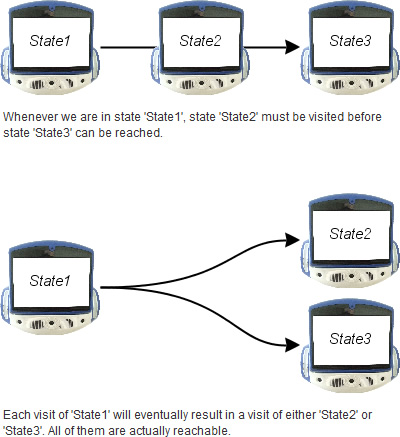
\includegraphics[scale=0.7]{templateconstraints}
  \caption{The two template constraint types, parameterized with particular states.}
  \label{fig:templateconstraints}
\end{figure}

\begin{figure}[htbp]
  \centering
  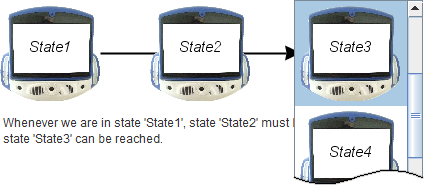
\includegraphics[scale=0.7]{templateconstraint_dropdown}
  \caption{Possible way of specifying template parameter.}
  \label{fig:templateconstraint_dropdown}
\end{figure}

All template constraints are additionally equipped with textual expressions in order to explain their semantics. It is a template sentence with placeholders for the states available for parameterisation. Whenever there is a change to the constraint, te text is being updated automatically regarding to the parameter states. These additional expressions are also shown in figure~\ref{fig:templateconstraints}.

Each template constraint describes a certain behaviour which might be later used for checks. Thus, specific formulas have to be provided which represent the semantics of the constraints. They have to be in a format so that they can be processed by a model checker. For the first kind of template operator, a linear temporal logic fomula (LTL, see~section~\ref{sec:modelcheckingandltl}) expresses its semantics (with $x$ as ``x is current state'' and similarly for $y$ and $z$):

\begin{equation} \label{eq:template_one}
  \models \Box (x \rightarrow ([(\neg z) \mathcal{U} y] \vee \Box \neg z))
\end{equation}

``Globally is true: Whenever x is the current state, either z is not visited until y or z is never visited''. Compared to the example above it means: Whenever a person eats something (x), he can not go to bed (z) until he brushes his teeth (y). Otherwise, if he never goes to bed, he does not necessarily need to brush his teeth.

The semantics of the second operator template is more complex since it has a secondary condition that all y, z, ... states are actually reachable after a visit of x. Possibilities can not be expressed by LTL, thus, it needs to use computation tree logic (CTL) for describing this auxiliary condition in a second formula. A short explanation about CTL is already given in section~\ref{sec:delbimbo}, but the two new constructs used for this formula are described below.
The main formula for the second template is still using LTL:
\begin{equation} \label{eq:template_two_one}
  \models \Box (x \rightarrow \Diamond (y \vee z (\vee ...)))
\end{equation}
``Globally is true: Whenever x is the current state, in a future step either y or z (or ...) will be visited''. In context of the example mentioned above it means: Every time a person enters a supermarket (x) he will eventually buy something (y) or buy nothing (z). The fact that both states are really potentially reachable is expressed by the following CTL formula. \emph{AG} replaces the $\Box$ sign and stands for ``on all paths is globally true...'', \emph{EF} is related to $\Diamond$ and expresses ``a path exists where is true in future...''.
\begin{equation} \label{eq:template_two_two}
  \models AG (x \rightarrow ((EF y) \wedge (EF z) (\wedge ...)))
\end{equation}
``It is globally true on all pahts: Whenever x is the current state, there is at least one path leading to y and at least one path leading to z''.








\section{Operator constraint formalism}
\label{sec:operatorconstraintformalism}

The operator constraint formalism is a new approach with a special focus on expressiveness and uniqueness of the visual language.
%For this the abstraction level is adapted in order to 
It is designed as a visual formalism for linear temporal logic having a visual operator for each LTL operator. Since the visual constraints are directly mapped to LTL expressions, the visual language is equal to LTL in expressiveness. If it is considered as easy to use, non-experts can use it as well as experts who already know LTL.


\subsection{Requirements}

To provide the required functionality, the fundamental logical operators are required, as shown in (a) through (e) below.

\begin{description}
	\item[(a)] \emph{AND} operator: $\varphi \wedge \psi$.\\This conjunction evaluates to true only when both $\varphi$ and $\psi$ are true.
	\item[(b)] \emph{OR} Operator: $\varphi \vee \psi$.\\At least one $\varphi$ or $\psi$ being true makes this construct true. The result is false when both parameters are false.
	\item[(c)] \emph{IF} operator: $\varphi \rightarrow \psi$.\\Instead of an \emph{IMPLIES} operator an \emph{IF} operator is provided. Its meaning seems to be more intuitive for non-experts since it is a common construct in almost every programming language.
	\item[(d)] \emph{NOT} operator: $\neg \varphi$. This operator negates the value of $\varphi$.
	\item[(e)] Proposition: $\rho$.\\Until now there is only the \emph{state proposition} type, which gives evidence about the currently active state. Other types such as numeric or string equations may be added but are less important for the healthcare subject.
\end{description}
	
In addition to these five logical operators the visual language should be furthermore capable of expressing constraints about future steps, both ``any future state'' (h) and ``the next state'' (g), that ``events should always happen'' (f), and that ``a property must be true until some future event'' (i).
	
\begin{description}
	\item[(f)] \emph{ALWAYS} operator: $\Box \varphi$.\\$\varphi$ must be true now and in all following states.
	\item[(g)] \emph{NEXT} operator: $\medcircle \varphi$.\\$\varphi$ has to be true in the next state.
	\item[(h)] \emph{FUTURE} operator: $\Diamond \varphi$.\\At least one time - now or in a later state - $\varphi$ must be true.
	\item[(i)] \emph{UNTIL} operator: $[\varphi \mathcal{U} \psi]$.\\Now and in all following states $\varphi$ must be true at least until there is a state with $\psi$ being true. In addition eventually there has to be a future state with $\psi$ being true.
\end{description}

All the operators mentioned above shall be suitable for constraint editing in a way that the visual language is very easy to use, especially for non-experts. This implies simple editing as well as easy readability of constraints. Furthermore it should provide an intuitive application which is ideally learnable within little time.





\subsection{Design decisions}
\label{sec:designdecisions}

Like the formula representation introduced by Del Bimbo et al.~\cite{520786}, a constraint consists of nested operators and propositions in a hierarchy. However, the new visual formalism surrenders the three dimensional idea and focuses on two dimensional blocks and their compositions instead, which is used by HomeTL~\cite{4341725} as well. Each operator of the visual language is represented by such a block.

The visual language has support for eight unary or binary operator types and one proposition which have their specific semantics. In order to support the reading of constraints, different significant visual appearances of the operator types shall enable easy classification and a faster subconscious identification~\cite{moody-physics-of-notations}. In this case, different colors are used for each operator type.
% aiming for faster perceptibility and understandability. 
A suggestion for the operators' graphical representation is shown in figure~\ref{fig:operators}.

\begin{figure}[htbp]
  \centering
  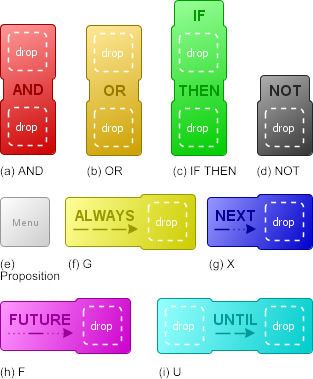
\includegraphics[scale=0.65]{table}
  \caption{Visual representation of all supported operators.}
  \label{fig:operators}
\end{figure}

A second effort for making the perceptibility of the visual language as intuitive as possible is done with the orientation of constraints. 
Operators which consist of nested operators have particular meanings for the two dimensions: The ``logical'' vertical read direction and the horizontal direction for variation in time. Thus, logical operators are arranged in a vertical row wereas time relevant operators are aligned horizontally.
Figure~\ref{fig:directions} demonstrates an example constraint composed along the logical and time axes.
\begin{figure}[htbp]
  \centering
  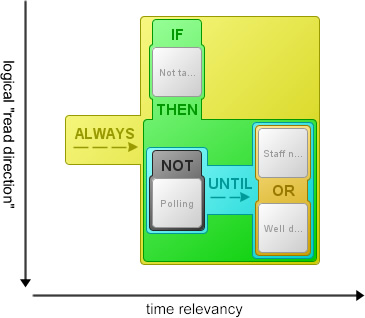
\includegraphics[scale=0.65]{directions}
  \caption{Easy understanding of visual constraints due to intuitive read directions.}
  \label{fig:directions}
\end{figure}
It is read from left to right and top to bottom:
``ALWAYS is true: IF state \emph{'Not taken yet'} is active THEN state \emph{'Polling'} can NOT be visited UNTIL state \emph{'Staff notified'} OR state \emph{'Well done!'} is reached.''

The two dimensions form a special requirement also for the layouting of nested operators. Each operator adapts its size so that it surrounds all recursively nested operators. But also the positioning of nested operators within teir parents have to be taken into account.
Whereas the operator's centered positioning and resizing along the logical direction only depends on the sizes of all sub operators, the arrangement within the time axis turns out to be more complex. Here, sub operators can not just be aligned centered as it is the case vertically. To face the determination of horizontal positioning, every operator gets time reference lines which specify its positioning within its parent and the positioning of its own children within itself. As depicted in figure~\ref{fig:referencelines}, logical operators - i.e. \emph{IfThenOperator}, \emph{AndOperator}, \emph{OrOperator}, \emph{NotOperator} and \emph{StateOperator} - have one reference line. Time relevant operators - i.e. \emph{NextOperator}, \emph{FutureOperator}, \emph{AlwaysOperator} and \emph{UntilOperator} - have two such reference lines, one for their own positioning within their parents and one for the positioning of their children.

\begin{figure}[htbp]
  \centering
  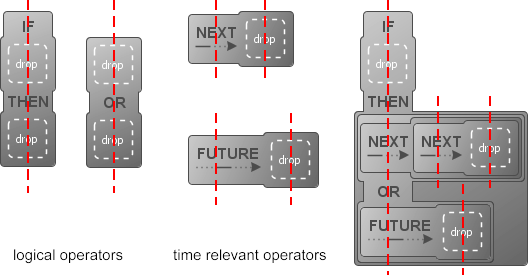
\includegraphics[scale=0.65]{referencelines} 
  \caption{Time reference lines and their adjustments.}
  \label{fig:referencelines}
\end{figure}

As postulated in the requirements for the visual language, constraints shall be easy to read. In fact, there is a possibility to improve the presentation of certain visual constraints. Multiple nested operators of the same kind which have no order priorities such as \emph{OR} or \emph{AND} appear graphically unnecessarily complex. These operators can be visually merged in the manner of unifying their border lines, for example. As a result, all associated operators appear as just one operator with a couple of sub operators (see~figure~\ref{fig:nested_and}).

\begin{figure}[htbp]
  \centering
  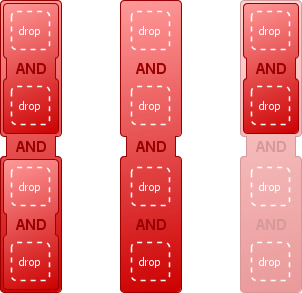
\includegraphics[scale=0.65]{and_simplify}
  \caption{Default nested \emph{AND} operator and visually merged nested \emph{AND} operator.}
  \label{fig:nested_and}
\end{figure}		







\subsection{Guidelines for an editor}

Also an editor for this visual language which holds the functionality for composing operators can contribute to usability and clarity. Some requirements are as follows:

\begin{itemize}	
	\item All editing is performed only by simple drag and drop. Operators and propositions can be moved and dropped onto other operators. A tool bar provides all operator and proposition types to be instantiated and a possibility for deleting existing operators.
	\item In order to simplify the reading of constraints an operator can be hovered over by the mouse pointer. It is intended to be similar to line coloring when reading a digital text.
	\item Every edit to either the constraint or the underlying state machine results in an automatically (re-)validation of the constraint. The result is immediately displayed to the user.
	\item There is no button for constraint creation / editing except operator and proposition providers, which let the developer create new instances. Having no additional buttons reduces complexity and keeps it simple.
\end{itemize}









\section{Comparison}
\label{sec:comparison}

Due to its arrow based design the visual language for template constraints is a good visualisation of time dependencies. Furthermore, it allows expressing possibilities by the use of CTL formulas which is not possible with the operator costraint formalism.
Nevertheless, the template visualisations have some trouble with clearness of their semantics. Even though there are well defined formulas behind each constraint and textual expressions which explain the meanings of constraints, the visual presentation seems to be ambiguous in some settings what leads to the risk of being interpreted differently. For example, in the context of the visual language it is unclear whether the first constraint template allows state (x) to be visited more than once before state (z) is reached. It might also be problematic to interprete whether more than one of the states $y$, $z$, ... can be actually visited after a visit of $x$ in the second constraint. In contrast, the operator constraint formalism is not ambiguous due to to its direct mapping to LTL wich is consistently defined. All visual operator expressions represent exactly the same semantics as their corresponding textual LTL formulas.

%The visual language for template constraints was presented to potential users for evaluation and feedback. Though most of them named it a good concept, soon it turned out that they had problems and disagreements concerning the issues mentioned above. The presented constraints were interpreted differently, the meaning seemed to be unclear and ambiguous. 

However, there is a second problem with the template constraints.
Whereas the safety constraints specific to the example within the healthcare domain mentioned in section~\ref{sec:healthbotapplication} are expressable by this visual language, there are other common constraints which have no matching template and thus can not be described. For example, the check of a state being visited never or at least once is not possible. For every new constraint type a new template has to be created what means an infinite amount of templates is needed in order to achieve full expressiveness.
On the contrary, the visual language for operator constraints is not limited in expressiveness compared to LTL, disregarding that there is only one proposition type available. But this is an extension issue of the prototype rather than a lack in expressiveness.
% Gefundene probleme, die man erw�hnen k�nnte: beim if operator ist das �bergeordnete always nicht intuitiv. der always operator k�nnte umgedreht sein.

Since a visual language has to be developed which suits non-professionals as well as experts, the risk of ambiguity is undesirable. Especially for a tool for safety and consistency it would form a really bad basis. For this reason, the approach of template constraints is discarded and the operator constraint formallism is used for the editor prototype instead.
Owing to the recursive nesting of operator constraints, a visual formula can be recursively translated to a LTL sentence which can be processed by the prototype using any ordinary model checker.
\chapter{Automated generation of safety constraints}
\label{chap:automatedgenerationofsafetyconstraints}

Safety constraints primarily constitute essential properties which describe correct and safe behaviour of safety critical software applications. In order to discover whether a program meets certain safety requirements, its behaviour is checked by the constraints. This happens mostly as a last check before software gets released. 
But regarding updating and maintenace work, often further changes are made to the software even after release.
%But even after possible changes to the software in the context of updating and maintenance work,
However, safety constraints can be applied again and assure the adherence of all properties. Safety constraints thus are also suitable for sustaining consistency during the different phases of software life. In fact, not only safety constraints, also properties of program behaviour which are not safety relevant at all are applicable for that. The more constraints are defined the better can be the reliability.
But as already mentioned before, it might be difficult for developers to find all reasonable %safety
constraints by hand. % which are needed for full safety covery.
In this case it can happen that a prior correct software version becomes faulty over time because of minor adjustments once in a while which are not covered by constraints.
%To help prevent this to happen

As a solution to this problem, the concept of automated constraint generation for state machines is proposed. Once the initial implementation of a program is finished, the behaviour of this state machine can be analyzed. In particular, heuristics can be elaborated which determine significant parts of the state machine automatically and put them into constraint representation. These constraints are of course valid on the current program.
On the one hand, the constraint suggestions may help the developer identifying reasonable constraints he did not think about as well as contradictions between program and specification, eg.\ if a computed constraint does not make sense at all.
On the other hand, all constraints can be revalidated after each change to the software and thus ensure consistency.

In order to support the developer in developing safe programs and to simplify maintainability, automated generation and suggestion of constraints for state machines might be helpful. But it is helpful only if the suggested constraints are relevant and reasonable.


\section{Subgraph definition}
\label{sec:subgraphdefinition}

Whether suggested constraints are relevant and reasonable
%This however
depends on the domain and use case. It has to be mentioned that the approach of finding an algorithm for constraint generation presented in this work has a special focus on the healtcare use cases and is not necessarily applicable for other domains.
Among others, each safety constraint postulated in chapter~\ref{chap:goals} was analyzed on a state machine program which represents the medication reminder application of the health care project. It turned out that all states which are named in the constraint are always connected in an identical manner and seem to fall into one of the following categories:

\begin{enumerate}
	\item States having two or more outgoing transitions ($\alpha$-states).
	\item States in which all paths starting from one $\alpha$-state come together again ($\beta$-states).
	\item All States immediately before $\beta$ states ($\gamma$-states).
\end{enumerate}

%All associated states which match these properties can be combined to a 
In order to compute the required constraints automatically, and possibly additional ones, for each $\alpha$-state all associated $\gamma$-states and the one $\beta$-state have to be determined. Such a group of states of a state machine is named subgraph from now on. It is defined as follows:
%Each $\alpha$-, the corresponding $\beta$- and several $\gamma$-states form a part of a state set called \emph{subgraph}. In order to retreive valid constraints a subgraph is defined by the following requirements: %as follows

\begin{itemize}
	\item There is a start state ($\alpha$-state) with at least two outgoing transitions.
	\item There is one end state ($\beta$-state) which is the first state where all possible paths of the state machine starting from start state come together again.
	\item All states between the start and end state also belong to the subgraph. They have no other incoming transitions than the ones originally coming from the start state. That means there is no path to visit these states except through the start state.
	\item The start state may have incoming transitions from states not contained in the subgraph.
	\item The end state may have self transitions or incoming and outgoing transitions from and to states which are not contained in the subgraph. Transitions back into the subgraph are not allowed except to the start state.
	\item Except self transitions of the end state, no cycles are allowed in the subgraph.
\end{itemize}

A graphical example of such a subgraph is shown in Fig.~\ref{fig:subgraph}. Using this specification all possible subgraphs of this kind can be detected within a state machine. An algorithm how subgraphs can be computed programmatically is discussed later in section~\ref{sec:prototype:automatedconstraintgeneration}.

\begin{figure}[htbp]
  \centering
  
  \tikzstyle{state} = [circle,fill=white,draw]
  \tikzstyle{statein} = [circle,fill=blue!20,draw]
  \tikzstyle{every path} = [font=\sffamily\small]
  
	\begin{tikzpicture}[->,>=stealth',shorten >=1pt,auto,node distance=15mm]
	
	
%	  \node[statein] (1) {$\alpha$};
%	  \node[state] (2) [above left of=1] {};
%	  \node[state] (3) [below left of=1] {};
%	  \node[statein] (4) [above right of=1] {};
%	  \node[statein] (5) [below right of=1] {};
%	  \node[statein] (8) [right of=5] {$\gamma$};
%	  \node[statein] (6) [right of=4] {$\gamma$};
%	  \node[statein] (7) [below right of=4] {$\gamma$};
%	  
%	  \node[statein] (9) [right of=7] {$\beta$};
%	  \node[state] (10) [above of=9] {};
%	  \node[state] (11) [above right of=9] {};
%	  \node[state] (12) [below right of=9] {};
%	  
%	  \path[dashed]
%	    (2) edge node [left] {} (1)
%	    (3) edge node [left] {} (1)
%	    (10) edge node [left] {} (9)
%	    (9) edge node [left] {} (11)
%	    (9) edge node [left] {} (12);
%		\path[]
%	  	(1) edge node [left] {} (4)
%	        edge node [left] {} (5)
%	    (4) edge node [left] {} (6)
%	        edge node [left] {} (7)
%	    (5) edge node [left] {} (8)
%	    (6) edge node [left] {} (9)
%	    (7) edge node [left] {} (9)
%	    (8) edge node [left] {} (9)
%	    ;
	    
	    
	  \node[statein] (1) {$\alpha$};
	  \node[state] (2) [above left of=1] {};
	  \node[state] (3) [above right of=1] {};
	  \node[statein] (4) [below left of=1] {};
	  \node[statein] (6) [below of=4] {$\gamma$};
	  \node[statein] (7) [below right of=4] {$\gamma$};
	  \node[statein] (5) [below right of=1] {};
	  \node[statein] (8) [below of=5] {$\gamma$};
	  \node[statein] (9) [below of=7] {$\beta$};
	  \node[state] (10) [right of=9] {};
	  \node[state] (11) [below left of=9] {};
	  \node[state] (12) [below right of=9] {};
	  
	  \path[dashed]
	    (2) edge node [left] {} (1)
	    (3) edge node [left] {} (1)
	    (10) edge node [left] {} (9)
	    (9) edge node [left] {} (11)
	    (9) edge node [left] {} (12);
		\path[]
	  	(1) edge node [left] {} (4)
	        edge node [left] {} (5)
	    (4) edge node [left] {} (6)
	        edge node [left] {} (7)
	    (5) edge node [left] {} (8)
	    (6) edge node [left] {} (9)
	    (7) edge node [left] {} (9)
	    (8) edge node [left] {} (9)
	    ;
	
	\end{tikzpicture}
  \caption{Example for a subgraph.}
  \label{fig:subgraph}
\end{figure}




\section{Constraint determination}
\label{sec:constraintdetermination}

For the healthcare applications, all important states which concern safety constraints belong to subgraphs. Thus, several safety properties can be formulated based on the structure of subgraphs.
For each subgraph the following valid LTL formulas can be derived if it contains neither inner (infinite) loops nor final states (states having no outgoing transition). In the following $\alpha$ is proposition for ``$\alpha$ is current state'' and similarly $\beta$ and $\gamma$:

\begin{equation} \label{eq:first}
  \models \Box (\alpha \rightarrow \Diamond \beta)
\end{equation}

\begin{equation} \label{eq:second}
  \models \Box (\alpha \rightarrow \Diamond (\bigvee_{\gamma} \gamma))
\end{equation}

\begin{equation} \label{eq:third}
  \models \Box (\alpha \rightarrow [\neg \beta \mathcal{U} \bigvee_{\gamma} \gamma])
\end{equation}

Additionally, for all states not contained in the subgraph (let's call them $\delta$-states, and the proposition $\delta$ stands for ``$\delta$ is current state'') the following formula is true: 

\begin{equation} \label{eq:fourth}
  \models \Box (\alpha \rightarrow [(\bigwedge_{\delta} \neg \delta) \mathcal{U} \beta])
\end{equation}

In case of $\alpha = \beta$ - i.e. when all paths starting from $\alpha$-state eventually return again (cycle) - even another constraint can be assumed to be true:

\begin{equation} \label{eq:fifth}
  \models \Box \Diamond \alpha
\end{equation}
 

These five constraints apply to each subgraph matching the conditions mentioned above. Formula~\ref{eq:first} says that an $\alpha$-state is always eventually followed by a $\beta$-state. Formula~\ref{eq:second} ensures that there will always at least one $\gamma$-state be eventually visited after each visit of an $\alpha$-state. The quite similar but stricter formula~\ref{eq:third} additionally demands a visit of at least one $\gamma$-state before the $\beta$-state can be reached. Formula~\ref{eq:fourth} simply says that a state not contained in the subgraph can not be visited between $\alpha$- and $\beta$-states. The constraint that the $\alpha$-state will always eventually be visited again is expressed by formula~\ref{eq:fifth}.

All formulas can be translated to the visual formalism presented in section~\ref{sec:operatorconstraintformalism} and shown to the user. The appropriate LTL formulas for the constraints postulated in chapter~\ref{chap:goals} relate to number \ref{eq:second} and \ref{eq:fifth} of the subgraph based formula templates and are as follows:

\begin{equation} \label{eq:sixth}
  \models \Box \Diamond \textnormal{'Polling'}
\end{equation}

\begin{equation} \label{eq:seventh}
	\models \Box (\textnormal{'Not taken yet'} \rightarrow \Diamond (\textnormal{'Well done!'} \vee \textnormal{'Staff notified'})
\end{equation}
%	\item The program will always eventually check the database for new reminder jobs. Thus we avoid that pending reminder are never processed.
%	\item Either a reminded medication is taken properly or caregivers get notified whenever a patient refuses medication intake.

Formula~\ref{eq:sixth} ensures that state ``Polling'' will always eventually be visited again, and formula~\ref{eq:seventh} specifies that either state ``Well done!'' or state ``Staff notified'' will be eventuelly visited after each visit of ``Not taken yet''.
\chapter{The LTLCreator prototype}
\label{chap:theltlcreatorprototype}

As stated in chapter~\ref{chap:goals}, appropriate support by a graphical editor is important for the usefulness of the developed visual language. Therefore a prototype of such an editor has been designed and implemented which contains the visual language as well as the proposed constraint generation heuristics. The implementation is a Java Swing component and has a simple API definition, making it easy to integrate the \emph{LTLCreator} tool into other java applications.

First of all the model implementation for representing state machines is described in section~\ref{sec:statemachinemodel}. Then, some details about the implementation of the visual language are given in section~\ref{sec:prototype:operatorconstraints}, directly followed by an explanation about the realization of the automated constraint generation functionality in section~\ref{sec:prototype:automatedconstraintgeneration}.
The assembly of all the previous features in one tool is described in section~\ref{sec:coalescence}. However, the tool's functionality shall also be available in Robostudio in order to provide safety mechanisms for the healthcare service robots and to be a prototype for evaluation. Section~\ref{sec:integrationintorobostudio} gives a main idea how an integration into Robostudio is possible. 


\section{State machine model}
\label{sec:statemachinemodel}

For the checking of constraints as well as for the constraint generation a model is needed which represents the state machine program. Three classes are responsible for holding the state machine program with all its necessary information: The class \emph{Fsm} represents the finite state machine and lists all contained states. It is called finite state machine, because the number of states is finite which applies to the domain of this work. \emph{State} represents the states of the machine and holds a list of all transitions from or to itself. Transitions are represented by the class \emph{Transition} which specifies the source and a target state. Figure~\ref{fig:fsm_class} shows all three class definitions for the state machine model.

\begin{figure}[htbp]
  \centering
  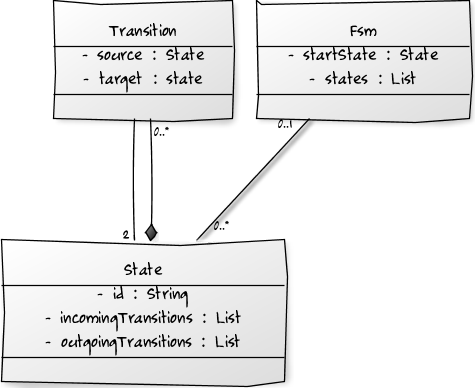
\includegraphics[width=0.65\linewidth]{fsm_class} 
  \caption{Class definitons for the state machine model.}
  \label{fig:fsm_class}
\end{figure}




\section{Operator constraints}
\label{sec:prototype:operatorconstraints}

All operator types, i.e. \emph{IfThenOperator}, \emph{AndOperator}, \emph{OrOperator}, \emph{NotOperator}, \emph{NextOperator}, \emph{FutureOperator}, \emph{AlwaysOperator}, \emph{UntilOperator} and \emph{StateOperator}, are realized by dedicated classes. All of them inherit from one abstract class \emph{AbstractOperator} which provides the basic functionality beeing used by all operators. The \emph{AbstractOperator} class is shown in figure~\ref{fig:abstractoperator} and its methods are described as follows:

\begin{description}
	\item[getLTL():] This function returns the LTL formula of an operator and all its children recursively. Applied to the most outer operator it returns the complete formula for the constraint. This function is abstract and implemented by each operator type separately.
	\item[getColor():] Each operator type has got is own significant color which can be retrieved by the abstract function \emph{getColor()}.
	\item[createNewInstance():] In order to provide operator creation over a tool bar, this function instantiates a new operator object, depending on the implementation.
	%\item[setMouseOver(boolean):] Mouse over actions cause the underlying operator to be highlighted. This function makes all operators except the hovered one appearing bleeched out.
	%\item[paintOperator(Graphics, ...):] Each operator class has to implement the abstract function \emph{paintOperator()}. It manages all color and shape painting for the respective operator. Additional parameters such as recursive painting including children can be specified.
	%\item[contains(int, int):] Given two coordinates x and y, it can be determined whether the herewith defined point lays within an operator.
	\item[isSimilar(AbstractOperator):] Two operators can be compared for semantic equality. Equality is given if the compared operators are of the same type and similarly their children. This functionality is important for avoiding duplicate constraints during constraint generation, for example.
	\item[addChangeListener(OperatorChangeListener):] Whenever there is a change to the operator or to one of its children, an operator change listener gets notified about it. The hierarchical architecture of \emph{AbstractOperator}s propagates all change events to the root operator. The function \emph{addChangeListener()} allows registering for such change notifications.
	\item[removeChangeListener(OperatorChangeListener):] According to \emph{addChangeListener} this function allows deregistration again.
\end{description}

\begin{figure}[htbp]
  \centering
  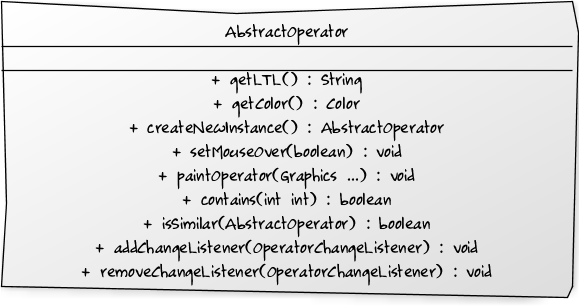
\includegraphics[width=0.6\linewidth]{AbstractOperator} 
  \caption{Class definition for \emph{AbstractOperator}.}
  \label{fig:abstractoperator}
\end{figure}

Whereas \emph{StateOperator}s have no operator children and are leafs in the syntax tree of LTL formulas, all other operator types are either unary or binary operators with one or two optional nested children respectively. 
The graphical representation of both unary and binary operators thus needs to have place holders and docking stations
\begin{wrapfigure}{r}{0.40\textwidth}
  \centering
  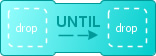
\includegraphics[scale=0.65]{bucket_example.jpg}
  \caption{Buckets for graphical nesting of operators.}
  \label{fig:bucket_example}
\end{wrapfigure}
for sub operators. These are realized by buckets which display a small ``drop'' label as shown in figure~\ref{fig:bucket_example} and allow operator adding or removing by mouse drops.
For this a class \emph{Bucket} is defined with get and set methods for defining a sub operator.
Figure~\ref{fig:klassendiagramm_operators} depicts the relationship between \emph{AbstractOperator}, \emph{Bucket} and operator implementations.
Once operators are composed in a way that no empty buckets are left over, a complete constraint such as the one shown in figure~\ref{fig:operator_tree} is retrieved. This diagram illustrates the correlation of nested operators and buckets.
\begin{figure}[htbp]
  \centering
  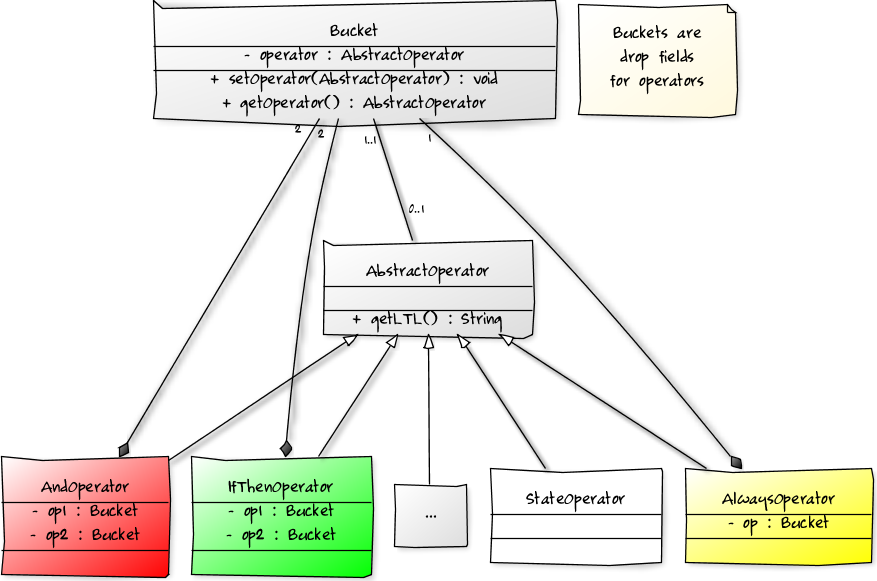
\includegraphics[width=\linewidth]{klassendiagramm_operators} 
  \caption{Class diagram of operator structure.}
  \label{fig:klassendiagramm_operators}
\end{figure}

\begin{figure}[htbp]
  \centering
  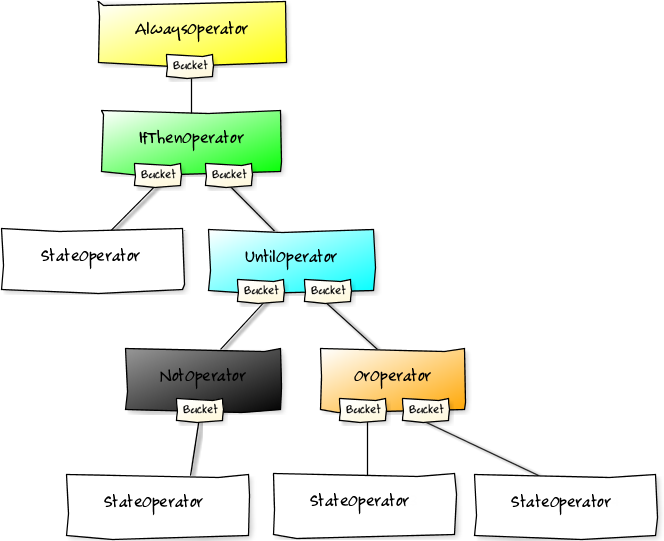
\includegraphics[width=0.95\linewidth]{operator_tree} 
  \caption{Instantiation of a constraint with several operators.}
  \label{fig:operator_tree}
\end{figure}

For the prototype implementation, all graphical components such as buckets and operators are implemented as Java Swing \emph{JComponent}. Thereby a lot of functionality for the visual configuration is already available such as the complex layout and repaint concept and the container functionality which is used for unary and binary operators as well as buckets.

%PAINT

Swing allows the implementation of a \emph{paint()} method which is responsible for rendering the component. This is used for giving every operator its special look. Swing's \emph{Graphics2D} functionality provides a great support in painting rounded shapes and color gradients. An operator is displayed as a rounded rectangle with dents around sub operators; it is displayed with a flowing backgound and borders and labels in the operator type's specific color. For the significant shape multiple rounded rectangles with and without borders are arranged in a way that the result appears to be one piece. Figure~\ref{fig:paintprocess} demonstrates how the process of painting works: For painting the \emph{IfThenOperator}, first of all a blank rectangle with border is drawn, directly followed by two filled rectangles with border which are placed where the two child operators shall be later on. In the third step the same rectangle as from step one is painted on top, this time without border. This makes all crossing borders disappear. Only labels and buckets still have to be added to create a complete \emph{IfThenOperator}.

\begin{figure}[htbp]
  \centering
  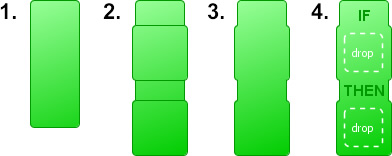
\includegraphics[scale=0.65]{paintprocess} 
  \caption{Four steps of painting an operator.}
  \label{fig:paintprocess}
\end{figure}

%LAYOUT

As proposed in the design decisions for the visual language in section~\ref{sec:designdecisions}, constraints have particular meanings for the two dimensions: A vertical read direction and the horizontal direction for variation in time. 
Swing's mechanism for layouting components is used for the positioning of operators. After determining the aspired sizes of child components which represent sub operators, reference lines which have been already demonstrated with figure~\ref{fig:referencelines} in section~\ref{sec:designdecisions} are computed mathematically. Based on this information operators are sized and positioned correctly.

%MOUSE OVER

Regarding to the requirement for simple reading of constraints based on mouse hovering, the editor prototype supports context sensitive highlighting of particular constraint parts.
The built-in mouse support of Swing is used for identifying the operator positioned under the mouse cursor. All operators except the hovered one and its sub operators are presented bleached out which causes the hovered operator to appear emphasized. The most right operator composition in figure~\ref{fig:nested_and_mouseover} gives a demonstration of this idea.

%PROBLEM WITH MOUSE OVER AND MERGING

However, the concept of operator highlighting causes trouble in combination with the graphical merging of visual operators which was introduced in section~\ref{sec:designdecisions}. Since a merged operator does not have its own border, it can not be displayed as desired when hovered. This fact is also a problem for the editing: The graphical presentation does not support changing of merged operators, because it seems that they can not be picked by the mouse.
In order to retain full editability, hovered operators are excluded from the merge rule and still have to be displayed separated (see~figure~\ref{fig:nested_and_mouseover}).
\begin{figure}[htbp]
  \centering
  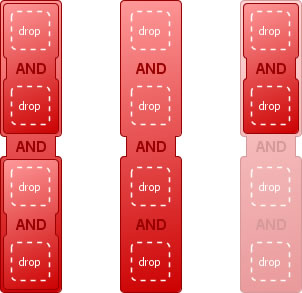
\includegraphics[scale=0.65]{and_simplify_mouseover}
  \caption{Default nested \emph{AND} operator, visually merged nested \emph{AND} operator and visually nested \emph{AND} operator with mouse over (from left to right).
  }
  \label{fig:nested_and_mouseover}
\end{figure}

%DRAG&DROP

Besides its importance for mouse hovering, Swing's mouse support is also used for determining the position where operators have to be added after drag and drop edit actions. So far
% the predefined Swing drag and drop has not been used but
a simple drag and drop mechanism called \emph{DndHandler} has been implemented whose class structure is shown in figure~\ref{fig:dndclassstructure}.
\begin{figure}[htbp]
  \centering
  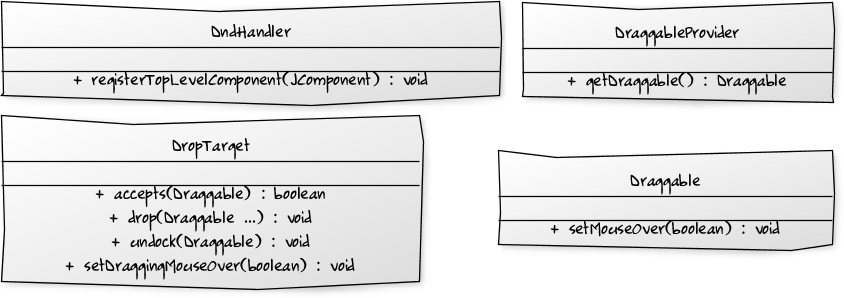
\includegraphics[width=\linewidth]{dndclassstructure} 
  \caption{Class definition for drag and drop functionality.}
  \label{fig:dndclassstructure}
\end{figure}% instead. 
Once a \emph{JComponent} is registered to the \emph{DndHandler}, it automatically manages any drag and drop actions with \emph{JComponent}s which implement either the \emph{Draggable} or \emph{DropTarget} interface. The former is implemented by all operators and specifies that this object can be moved from and to buckets or the dashboard, the latter is implemented by buckets and the dashboard and determines that it can accept and contain \emph{Draggable}s such as operators.
%Figure~\ref{fig:dndclassstructure} gives a short class overview.
Furthermore there is a class \emph{DraggableProvider} which is similar to \emph{Draggable} except that it is not moved itself but creates a new instance of the respective \emph{Draggable} implementation type which is then moved instead.

%TOOLBAR

\emph{LTLCreator} is equipped with a tool bar which provides all functionalities needed for constraint editing: For each operator type a \emph{DraggableProvider} is displayed as an icon in the respective operator color. Each time the mouse is pressed on it (drag action start), a new instance of the respective operator type is created which can be moved and dropped to the dashboard. Additionally, a trash can icon is displayed within the tool bar. It implements the \emph{DropTarget} interface and can thus receive operators. Its purpose is to provide a remove functionality for already instantiated operators which are not needed anymore.









\section{Automated constraint generation}
\label{sec:prototype:automatedconstraintgeneration}

As stated in section~\ref{sec:subgraphdefinition}, the automated generation of constraints for a state machine is based on subgraphs. For the finding of such subgraphs an algorithm has been developed. Section~\ref{sec:subgraphfindingconcept} aims to explain the basic concept of the algorithm, section~\ref{sec:subgraphfindingimplementation} introduces the slightly modified algorithm which is used for the prototype.
%It is described as follows:


\subsection{Subgraph finding concept}
\label{sec:subgraphfindingconcept}

First of all a start state ($\alpha$) is defined which has two or more outgoing transitions. All possible paths are generated which start from it and lead through the state machine. Every path ends before it visits states twice.
The result is a finite set of finite paths since loops are eliminated. Now every state gets as label assigned a number which represents the total number of occurrences of this state in all collected paths. In other words, the label of a state expresses the number of paths which start in the $\alpha$-state and contain this state. The $\alpha$-state itself is labeled with the total number of paths. If during walking through any of the paths a second state can be found with the same label, it means that all paths starting at $\alpha$-state come all together in this state again. It is determined to be a potential corresponding end state ($\beta$).
A last check has to be applied whether there are incoming transitions from outside into the subgraph which do not originally come from $\alpha$-state. If no such transitions are detected, a subgraph is found.
If there is no state with the same label, or a transition exists which comes from outside, the state machine as a whole can be assumed as subgraph beginning with $\alpha$-state insofar as the state machine does not contain further loops or terminating end states. Figure~\ref{fig:subgraph_finding} illustrates this concept of subgraph finding and shows all possible paths as well as the number of occurrences of each state.
\begin{figure}[htbp]
  \centering
  
  \tikzstyle{state} = [circle,fill=white,draw]
  \tikzstyle{statein} = [circle,fill=blue!20,draw]
  \tikzstyle{none} = [fill=white]
  \tikzstyle{highlighted} = [fill=yellow]
  \tikzstyle{every path} = [font=\sffamily\small]
  
	\begin{tikzpicture}[->,>=stealth',shorten >=1pt,auto,node distance=15mm]
	
	  \node[state] (1) at (0,0) {A};
	  \node[state] (4) [below left of=1] {B};
	  \node[state] (6) [below of=4] {D};
	  \node[state] (7) [below right of=4] {E};
	  \node[state] (5) [below right of=1] {C};
	  \node[state] (8) [below of=5] {F};
	  \node[state] (9) [below of=7] {G};
	  \node[state] (11) [below left of=9] {H};
	  \node[state] (12) [right of=9] {I};
	  
	  \node[state] (101) at (3,0) {A};
	  \node[state] (102) [below of=101] {B};
	  \node[state] (103) [below of=102] {D};
	  \node[state] (104) [below of=103] {G};
	  \node[state] (105) [below of=104] {H};
	  
	  \node[state] (201) at (4.5,0) {A};
	  \node[state] (202) [below of=201] {B};
	  \node[state] (203) [below of=202] {D};
	  \node[state] (204) [below of=203] {G};
	  \node[state] (205) [below of=204] {I};
	  
	  \node[state] (301) at (6,0) {A};
	  \node[state] (302) [below of=301] {B};
	  \node[state] (303) [below of=302] {E};
	  \node[state] (304) [below of=303] {G};
	  \node[state] (305) [below of=304] {H};
	  
	  \node[state] (401) at (7.5,0) {A};
	  \node[state] (402) [below of=401] {B};
	  \node[state] (403) [below of=402] {E};
	  \node[state] (404) [below of=403] {G};
	  \node[state] (405) [below of=404] {I};
	 
	  \node[state] (501) at (9,0) {A};
	  \node[state] (502) [below of=501] {C};
	  \node[state] (503) [below of=502] {F};
	  \node[state] (504) [below of=503] {G};
	  \node[state] (505) [below of=504] {H};
	  
	  \node[state] (601) at (10.5,0) {A};
	  \node[state] (602) [below of=601] {C};
	  \node[state] (603) [below of=602] {F};
	  \node[state] (604) [below of=603] {G};
	  \node[state] (605) [below of=604] {I};
	 
	  \node[highlighted] (701) at (12,0) {A=6};
	  \node[none] (702) at (12,-0.6) {B=4};
	  \node[none] (703) at (12,-1.2) {C=2};
	  \node[none] (703) at (12,-1.8) {D=2};
	  \node[none] (703) at (12,-2.4) {E=2};
	  \node[none] (703) at (12,-3.0) {F=2};
	  \node[highlighted] (703) at (12,-3.6) {G=6};
	  \node[none] (703) at (12,-4.2) {H=3};
	  \node[none] (703) at (12,-4.8) {I=3};
	  
		%\draw[->] (0, 0) .. controls(1,1) .. (3, 0);
		\draw[->] (12) to [out=45, in=0] (1);
	
	  \path[]
	  	(1) edge node [left] {} (4)
	        edge node [left] {} (5)
	    (4) edge node [left] {} (6)
	        edge node [left] {} (7)
	    (5) edge node [left] {} (8)
	    (6) edge node [left] {} (9)
	    (7) edge node [left] {} (9)
	    (8) edge node [left] {} (9)
	    (11) edge [bend left] node [left] {} (9)
	    (9) edge [bend left] node [left] {} (11)
	    (9) edge node [left] {} (12)
		  
		  
		  (101) edge node [left] {} (102)
		  (102) edge node [left] {} (103)
		  (103) edge node [left] {} (104)
		  (104) edge node [left] {} (105)
		  
		  (201) edge node [left] {} (202)
		  (202) edge node [left] {} (203)
		  (203) edge node [left] {} (204)
		  (204) edge node [left] {} (205)
		  
		  (301) edge node [left] {} (302)
		  (302) edge node [left] {} (303)
		  (303) edge node [left] {} (304)
		  (304) edge node [left] {} (305)
		  
		  (401) edge node [left] {} (402)
		  (402) edge node [left] {} (403)
		  (403) edge node [left] {} (404)
		  (404) edge node [left] {} (405)
		  
		  (501) edge node [left] {} (502)
		  (502) edge node [left] {} (503)
		  (503) edge node [left] {} (504)
		  (504) edge node [left] {} (505)
		  
		  (601) edge node [left] {} (602)
		  (602) edge node [left] {} (603)
		  (603) edge node [left] {} (604)
		  (604) edge node [left] {} (605)
		  ;
	
	\end{tikzpicture}
  \caption{Example for the subgraph finding algorithm: The occurrence labels of the states lead to
   %of each state in the paths lets you determine 
   G as an end state ($\beta$) corresponding to A.}
  \label{fig:subgraph_finding}
\end{figure}
This procedure is suitable for checking whether a state is the beginning of a subgraph and for discovering the corresponding $\beta$-state. In order to detect all subgraphs within a state machine, this procedure has to be applied to every single state which has two or more outgoing transitions. In order to improve the further finding of subgraphs and walking through the state machine, all already found subgraphs can be assumed as single states since it is already known where their paths come finally together again.%: In their $\beta$-states.



\subsection{Subgraph finding implementation}
\label{sec:subgraphfindingimplementation}

Following the previous description an algorithm has been implemented in Java. Its realization differs from the presented concept: Paths are not listed but states are directly labelled since not saving all possible paths is more memory efficient.
The state machine is traversed similarly to a depth-first search and each visited state's label is incremented by one. If the current state holds more than one outgoing transition and thus constitutes new paths,  all states on the current stack, i.e. the previously visited states on the current path, get their labels incremented by ('number of outgoing transitions' - 1). The algorithm turns back whenever it comes across a state which has already been visited within the same path stack of the depth-first search.

The overall implemented way of subgraph finding is illustrated in pseudo code with algorithm~\ref{alg:subgraphfinding}.
\begin{algorithm}
\caption{Finding of all subgraphs.}
\label{alg:subgraphfinding}
\begin{algorithmic}[1]
\STATE $subgraphs$: List
\FORALL{states as $S$}
  \STATE $start \leftarrow S$
	\STATE doLabelling($start$);
	\IF{state $E$ exists with label($E$)$=$label($S$)}
		\STATE $end \leftarrow E$
	\ELSE
		\STATE $end \leftarrow start$
	\ENDIF
	\IF{noCycles($start$, $end$) $and$ noExtTransitions($start$, $end$)}
		\STATE $subgraphs$.add($start$, $end$);
	\ENDIF
\ENDFOR
\end{algorithmic}
\end{algorithm}
Line 1 defines a variable $subgraphs$ which will contain all results of the algorithm after execution.
In line 4 the labelling process described above is executed by using one particular start state. Line 5 checks whether there is a state having the same label as the start state. If so, it is assumed as potential end state (line 6). Otherwise, the entire state machine is assumed to be a subgraph and the start state is defined as end state as well (line 8). Subsequent checks in line 9 finally determine whether it can be considered as proper subgraph.
There are no cycles allowed between start and end state since they are forbidden by the subgraph definition in section~\ref{sec:subgraphdefinition}.
Furthermore also foreign transitions are prohibited: Transitions coming from a state outside the subgraph are allowed to lead to the start state or the end state but not to other states of the subgraph. If all checks are successful, start and end states get added to the result list $subgraphs$ in line 11. This procedure is applied to all states of the state machine by the surrounding foreach loop (line 2). In the end, the list $subgraphs$ contains all pairs of start and end states which form subgraphs.


\subsection{Constraint generation}

After determining a subgraph, constraints are derived from it as defined in section~\ref{sec:constraintdetermination}. The entire process of constraint generation is illustrated by figure~\ref{fig:processofconstraintgeneration}.
\begin{figure}
  \centering

  \begin{sequencediagram}
		\tikzstyle{inststyle}+=[top color=yellow!30,bottom
color=white]
		\newthread{u}{User/Editor}{blue}
		\newthread[2.6]{cc}{Constraint creator}{red}
		\newinst[1]{alg}{Subgraph finding algorithm}

		\mess{u}{start(stm)}{cc}
		\begin{call}[3]{cc}{start(stm)}{alg}{finish}
			\begin{sdblock}[yellow!20]{For each subgraph}{}
				\setthreadbias{east}
				\begin{call}[3]{alg}{newSubgraph(subgraph)}{cc}{}
					\begin{sdblock}[yellow!20]{For each constraint}{}
						\begin{call}[3]{cc}{newConstraint(constraint)}{u}{}
						\end{call}
					\end{sdblock}
				\end{call}
				\setthreadbias{center}
			\end{sdblock}
		\end{call}
		\mess{cc}{finish}{u}
	\end{sequencediagram}
  
  \caption{Process of constraint generation.}
  \label{fig:processofconstraintgeneration}
\end{figure}
Once the user triggers the constraint generation for a state machine (stm), the subgraph finding algorithm starts working. When a subgraph is found, constraints are created and passed to the user. For each subgraph multiple constraint types can apply. This procedure is done iterative for each subgraph found.



The runtime of the algorithm depends on size and grade of branching of the state machine. An estimation about the execution time is presented later in section~\ref{sec:performance}. In order to improve waiting times and thus user experience during constraint generation the entire result might not be returned after termination but each subgraph should be processed as soon as it is found.
For this, the implementation for the algorithm has been extended by code snippets which frequently interact with so called \emph{ResultListener}s (figure~\ref{fig:resultlistener_class}).
%This interface is also implemented by the progress dialog.
An implementation of \emph{ResultListener} has to provide three methods which allow the algorithm to publish the current progress by calling \emph{void setProgress(int)} or to notify about newly found subgraphs by invoking \emph{void newSubGraphFound(SubGraph)}. The method \emph{boolean continueGeneration()} is called frequently and the execution will terminate as soon as it returns false.
\begin{figure}[htbp]
  \centering
  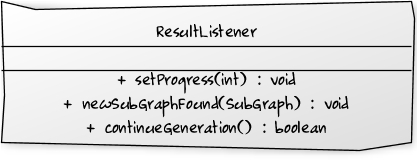
\includegraphics[width=0.50\linewidth]{resultlistener_class} 
  \caption{Interface definition of \emph{ResultListener}.}
  \label{fig:resultlistener_class}
\end{figure}

As a second approach aiming for better user experience during constraint generation, a dialog has been implemented which informs the developer continuously about the current progress. This includes the number of constraints found so far and a progress bar which gives a percentual estimation of execution time. Furthermore a cancel button permits premature stopping of the execution. A snapshot of the Dialog is shown in figure~\ref{fig:progressdialog}.
\begin{figure}[htbp]
  \centering
  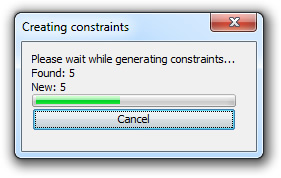
\includegraphics[width=0.34\linewidth]{progressdialog} 
  \caption{Snapshot of the progress dialog displayed during constraint generation.}
  \label{fig:progressdialog}
\end{figure}





\section{The LTLCreator}
\label{sec:coalescence}

Both features, the editor for the visual language presented in section~\ref{sec:operatorconstraintformalism} and the automated constraint generation in chapter~\ref{chap:automatedgenerationofsafetyconstraints}, were assembled in one tool, the \emph{LTLCreator}.
Figure~\ref{fig:LTLCreator} shows the assembled parts of \emph{LTLCreator}: A dashboard is provided where constraints can be edited visually by the developer and result displays indicate the validation results of constraints graphically. For validating the constraints an external model checker is linked to \emph{LTLCreator}. This component does not have an UI as well as the constraint generator, which is also part of \emph{LTLCreator}. 
\begin{figure}[htbp]
  \centering
  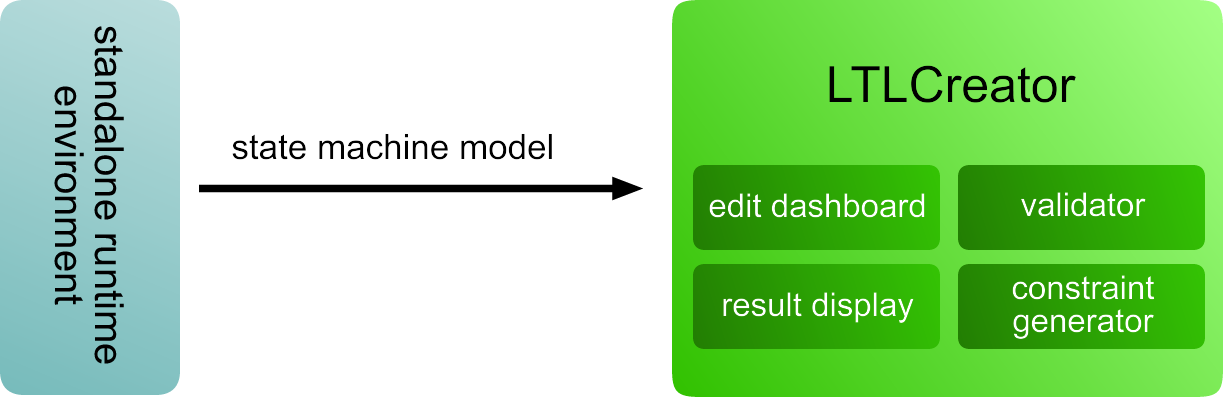
\includegraphics[width=0.65\linewidth]{LTLCreator}
  \caption{Integration of LTLCreator.}
  \label{fig:LTLCreator}
\end{figure}
The \emph{LTLCreator} itself does not provide functionalities for editing state machines although a state machine model is needed for the visual language as well as for constraint generation. Therefore the standalone version of \emph{LTLCreator} uses a hard coded state machine as model which represents an example program for test purpose.

Figure~\ref{fig:editor} shows a snapshot of the editor's environment:
\begin{figure}[htbp]
  \centering
  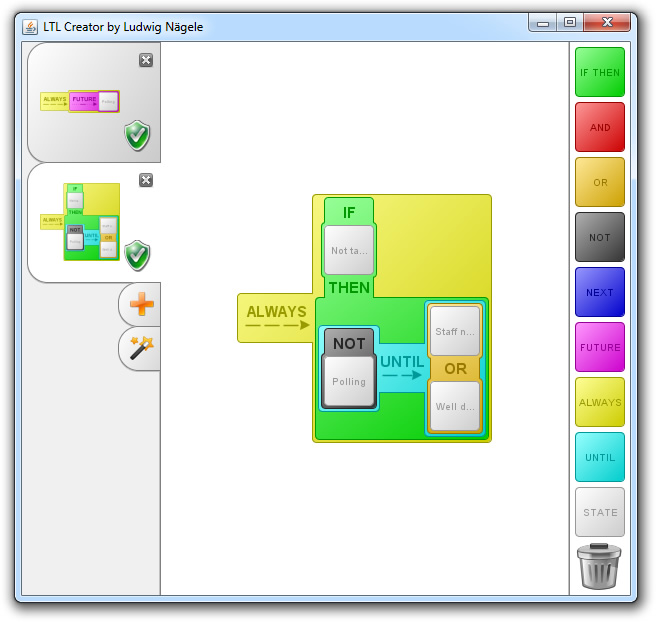
\includegraphics[width=\linewidth]{editor} 
  \caption{Snapshot of the visual editor LTLCreator.}
  \label{fig:editor}
\end{figure}
All functionalities needed for constraint editing are provided in the tool bar on the right (1). It contains draggable elements for creating all operator and proposition types as well as a trash can for deleting. Constraints can be composed by drag\&drop in the dashboard in the center of the editor (2) which holds and displays the operator constraints. The tab functionality on the left allows multiple constraints to be managed (3). Each tab shows a small thumbnail of the constraint and a symbol indicating its current status of validation result: For syntactically invalid constraints, an ``incomplete'' sign is displayed. Otherwise, an animated ring indicates that validation is in pro\-gress and will finally result in either a ``valid'' or ``invalid'' sign as shown in figure~\ref{fig:results}.
\begin{figure}[htbp]
  \centering
  
\includegraphics[scale=0.7]{results}
  \caption{Status indicators displaying validation results: incomplete, validation in pro\-gress, invalid and valid.}
  \label{fig:results}
\end{figure}
The magic wand button within the tab pane makes the constraint generation functionality accessible within the editor and triggers the constraint finding process.



\subsection{Model checker}

A main requirement to the \emph{LTLCreator} tool is that all constraints can be validated immediately and allow fast feedback about the correctness of programs. For this a \emph{ConstraintValidator} class has been defined which provides a method \emph{validate(AbstractOperator)} for proving constraints.
For the constraint validation itself a particular model checker can be specified. As a default, the symbolic model checker NuSMV~\cite{springerlink:10.1007/s100090050046,NuSMV2} is used. It is an open source project and has been designed to be an open architecture for model checking. NuSMV does not have a Java API but it can be externally accessed over command line. For this both the state machine program and the LTL formulas have to be translated to an input file which has to match a NuSMV specific format. For LTL formulas NuSMV uses the char ``G'' (for globally) instead of $\Box$ and the char ``F'' (for future) instead of $\Diamond$. An example of this input language is given in listing~\ref{lst:nusmv}.

\lstset{
  basicstyle=\ttfamily,
  columns=fullflexible,
  showstringspaces=false,
  commentstyle=\color{gray}\upshape
}
\begin{lstlisting}[float = htbp, captionpos=b, breaklines=true, showspaces=false, showtabs=false, tabsize=2, caption=Example of a NuSMV diagram file., label=lst:nusmv]
MODULE main
  VAR
    state: 1..11;
  ASSIGN
    init(state) := 2;
    next(state) := case state = 2 : {3, 1};
                          state = 3 : 1;
                          state = 1 : {2, 4};
                          state = 4 : {1, 5};
                          state = 5 : {6, 9, 10};
                          state = 6 : {7, 8};
                          state = 7 : 8;
                          state = 8 : 1;
                          state = 9 : 11;
                          state = 10 : {9, 11};
                          state = 11 : 1;
                          TRUE : state;
                     esac;

LTLSPEC G (state = 5 -> (F (state = 8 | state = 11)))
\end{lstlisting}
A state machine is encoded in the variable \emph{state}, and its value represents the active state. Thus, each state is identified by a number. The state machine described in the example of listing~\ref{lst:nusmv} contains eleven states, this is determined by the number range for \emph{state} from one to eleven. All variable assignments are specified under \emph{ASSIGN} and represent the semantic equivalent to transition definitions. The initial state can be determined and a case distinction regulates the next possible values, i.e. transitions to reachable states. If there are more than one outgoing transition, all target state identifiers have to be surrounded by brackets. The last expression \emph{TRUE : state;} is a self transition for every state not considered in the case distinction.
The last line contains the constraint formula which has to be checked on the state machine. The prefix \emph{LTLSPEC} just says that NuSMV has to interprete the following constraint as LTL formula.

This kind of output is generated by the \emph{ConstraintValidator} whenever a constraint needs validation. All states are then mapped to numbers and transitions get transformed into case distinctions. The result is stored to a file and then loaded by NuSMV. The corresponding valdidation result can be subsequently read from the command line and displayed in the editor next to the visual constraint. Due to issues of this command line API, each constraint is checked in a new NuSMV instance.

Model checking can be a quite ressource inefficient activity and due to high temporary data generation for each check, a parallel execution of multiple checks might overload the main memory which causes slow data swapping to start. This phenomen causes the overall execution to significantly slow down even on modern multicore CPUs since every process or thread has to wait for the memory. To avoid this it might be recommended to execute all validation tasks consecutively rather than in parallel.
However, it can happen that there is more than one validation task at a time. This is the case when the constraint generator creates multiple constraints in succession or a change of the state machine causes all constraints to be revalidated at once.
%An extra advantage is that the developer does not have to wait for all tasks to finish before he can see any result.
%Since a validation task is not startet until the previous one is finished, constantly new validation results can be displayed to the developer.
In order to avoid the concurrent execution of multiple NuSMV instances, the \emph{ValidatorThread}, a queue based mechanism for scheduling validations, manages a sequential processing of all validation tasks. Its class definition is presented in figure~\ref{fig:validatorthread_class}.
\begin{figure}[htbp]
  \centering
  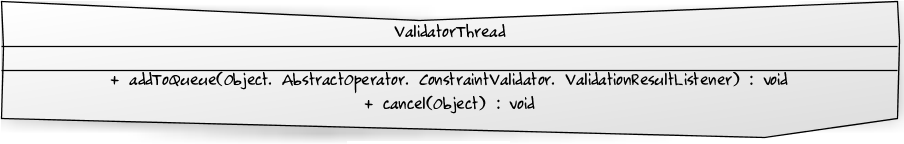
\includegraphics[width=\linewidth]{validatorthread_class} 
  \caption{Class definition of \emph{ValidatorThread}.}
  \label{fig:validatorthread_class}
\end{figure}
Every validation task of a constraint gets enqueued in the \emph{ValidatorThread} after calling the method \emph{addToQueue(...)}.
An identifier is used for each constraint which enables elimination of duplicate tasks for the same constraint in order to minimize the execution time. Tasks can also manually be removed from the queue by calling \emph{cancel(...)}. After a validation task is finished the result is published via callback to the \emph{ValidationResultListener}.









\subsection{External interface of LTLCreator}
\label{sec:easeofintegration}

\emph{LTLCreator} should be integratable into other state machine based programming environments. This is ensured by its implementation as a Java Swing component and a clear API which enables a wide range of use for this tool.

Figure~\ref{fig:coalescence} points out interactions between \emph{LTLCreator} and programming environments it is integrated in.
\begin{figure}[htbp]
  \centering
  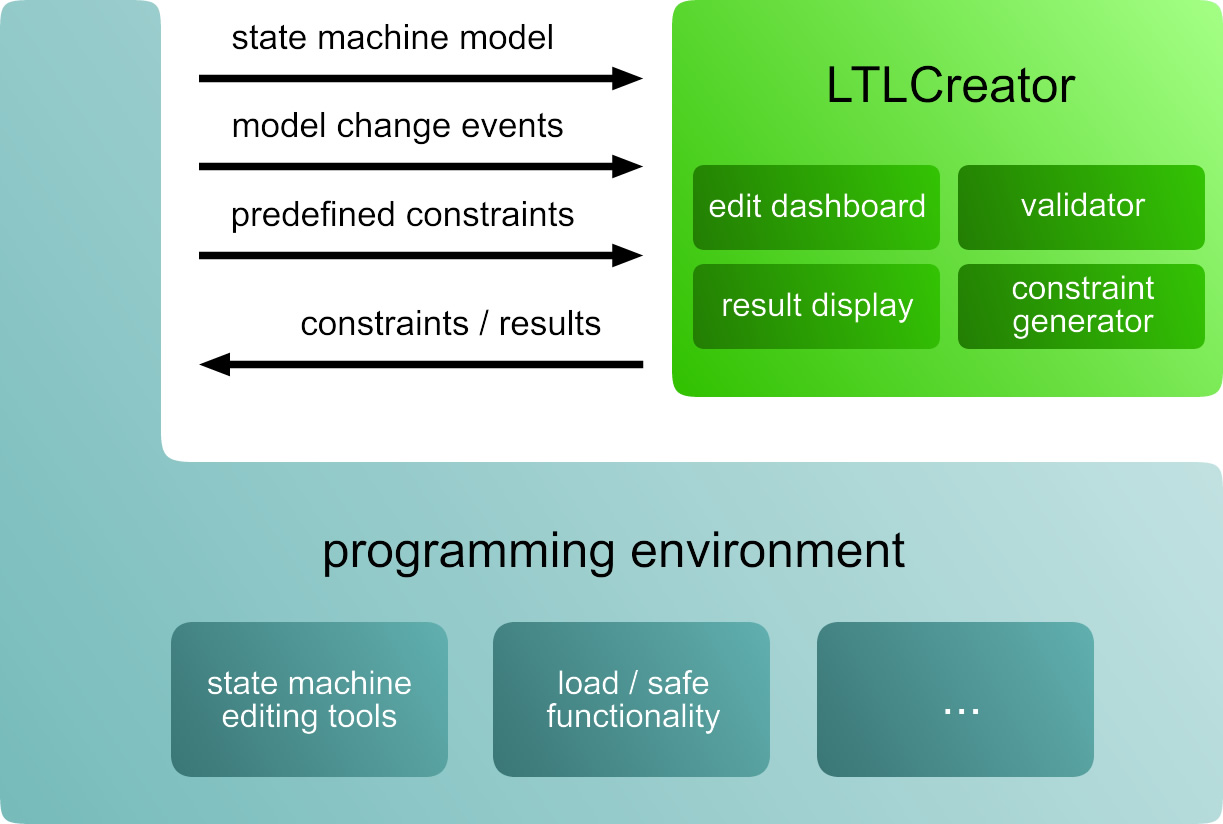
\includegraphics[width=0.7\linewidth]{coalescence}
  \caption{Interaction between LTLCreator and programming environment.}
  \label{fig:coalescence}
\end{figure}
The programming environment provides the state machine model and notifies the \emph{LTLCreator} component about all changes made to the model. This will automatically revalidate all existing constraints and always hold the up-to-date model for constraint generation.
For load and save functionality, all existing constraints can be received and new ones can be added to the \emph{LTLCreator} component programmatically.
All this functionality can be accessed through methods provided by the component \emph{LTLCreator}. Its class definition is shown in figure~\ref{fig:ltlcreator_class}. Whenever there is a change to the state machine, \emph{setModel(Fsm)} has to be called with the current state machine as parameter. This will cause the editor to revalidate where necessary. Constraint exchange can be done by using the methods \emph{addNewDashboard(AbstractOperator, ...)} and \emph{getOperators()}.

\begin{figure}[htbp]
  \centering
  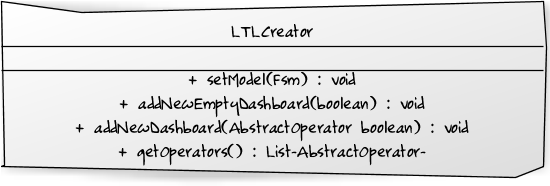
\includegraphics[width=0.65\linewidth]{ltlcreator_class}
  \caption{Class definition for \emph{LTLCreator}.}
  \label{fig:ltlcreator_class}
\end{figure}







\section{Integration into Robostudio}
\label{sec:integrationintorobostudio}

As stated in the previous section, the \emph{LTLCreator} provides an API for integration into other Java based applications. Robostudio,
a visual programming environment for rapid authoring and customization of complex services on a personal service robot, is such an application which was used for evaluating the visual language as well as the automated constraint generation feature and is also supposed to provide all this functionality for development of service robot behaviour in future.

Robostudio uses NetBeans~\cite{netbeans} as a platform and organizes all tools and features in windows. Thus also \emph{LTLCreator} was put into a window and added to the Robostudio platform. This was done by placing it into a NetBeans module which was added to Robostudio's modules. This module imports the \emph{LTLCreator} tool, archived as a jar file, and further consists of only two classes: \emph{LTLCreatorTopComponent} and \emph{XmlDataToLTLEditorDataWrapper}. The former implements the \emph{TopComponent} provided by NetBeans which can be used for displaying UI elements. In order to visualize the \emph{LTLCreator} component it is directly placed on the \emph{LTLCreatorTopComponent}. It retrieves changes of the model and passes them to the \emph{LTLCreator} component. Since the defining of safety constraints is an important issue not only after but also during the process of developing service robot behaviour, the \emph{LTLCreator} window as a vital tool has been positioned in the center of the platform where also the \emph{UI Component Layout Editor Window} is located.
The \emph{XmlDataToLTLEditorDataWrapper} forms the bridge between Robostudio's own model and the state machine model used by \emph{LTLCreator}. All complex data coming from Robostudio has to be cleaned from unimportant layout information and transformed to an elementary state machine representation before it can be processed by \emph{LTLCreator}.



%TODO: load and save



\subsection{Problems}

As already proposed in section~\ref{sec:easeofintegration}, all changes to the state machine program made within Robostudio must of course cause the \emph{LTLCreator} module to revalidate all existing constraints. This demands a concept of change notification management which is responsible for receiving all changes and making this information available for the \emph{LTLCreator} component. As a solution, all parts of the code where model changes are made should be extended with short code snippets which send notifications.
However, this is not as easy to realize in Robostudio since some of the relevant code was generated or even imported as external jars which makes code manipulation impossible.

A second challenge is the current data handling policy in Robostudio. Since this platform is mainly made for developers who used to edit RBDL xml code manually, Robostudio aims for visual rapid editing rather than for syntax checks. Thus, syntax errors are not detected or even ignored by methods like static analysis or input restrictions. In fact, such features have not been requirements for Robostudio. During integration of \emph{LTLCreator} into Robostudio problems came up when loading already existing RBDL programs of the healthbot project: Transitions leading to non existing states, transitions leading to nowhere (null) or transitions whose target is depending on runtime facts.
This characteristic seems to be a problem for the \emph{LTLCreator} which needs a complete and correct state machine as input and does not know how to cope with inconsistent data retrieved from Robostudio.




\subsection{Solutions}

To guarantee that all model changes cause the constraints to be revalidated, all relevant code parts have to report on this. But modification of the code has not been possible in all cases. Whereas all state changes are announced, transition changes stay unnoticed. This decision is sufficient for the prototype, but the developers of Robostudio announced an adapted architecture to solve this problem in the next version.


The problem with inconsistent data could be solved by plausibility and syntax checks during the transformation process of \emph{XmlDataToLTLEditorDataWrapper}. After successful transformation the state machine is passed to the \emph{LTLCreator} component. Otherwise no validation result is displayed for constraints and a dialog lists all identified syntax errors. In the context of safety and reliability a restrictive approach which gives no result at all seemed more applicable than an attempt to interpret the inconsistent data. 
\chapter{Test scenario and evaluation}
\label{chap:testscenarioandevaluation}

Both, the visual language and the automated constraint generation functionality, have been integrated into Robostudio in order to evaluate the proposed safety functionality. Robostudio is a visual programming environment which allows the specification of state machine based programs whose behaviour can then be examined by visual constraints.
As a test scenario the simplified medication reminder application is considered whose underlying screen-flow is explained in figure~\ref{fig:medicationreminder}. Starting from ``Menu'' the user can choose from several services such as blood pressure measurement or entertainment. In the given example these services are simplified to just one state ``additional services'' since the focus concentrates on the medication reminder part. In state ``Polling'' the database is checked for a pending reminder and, if there is one, the medication intake guidance is triggered. The patient can state if he or she has already taken the medication, or decide whether to take it or not. In the latter case, he or she may give a reason for it and a caregiver is notified about this incident. Otherwise the progress will result in the state ``Well done!'' after completing intake.

\begin{figure}[htbp]
  \centering
  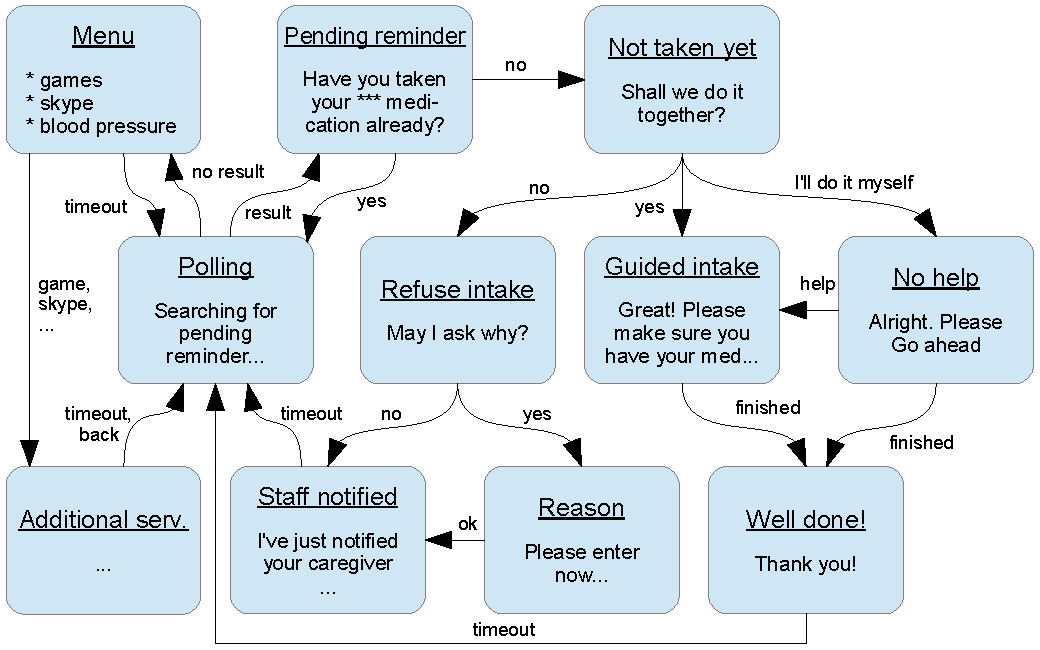
\includegraphics[width=\linewidth]{stm.pdf}
  \caption{Simplified screen-flow of the medication reminder application.}
  \label{fig:medicationreminder}
\end{figure}

This state machine with all its states, transitions and screen dialogs has been implemented in Robostudio and in the following sections~\ref{sec:testscenarioandevaluation_operatorconstraints} and~\ref{sec:testscenarioandevaluation_automatedconstraintgeneration} the visual language as well as the potential of constraint generation shall be evaluated. Section~\ref{sec:practicalexperiences} describes how a non-expert deals with the visual language and what the final judgement is.



\section{Operator constraints}
\label{sec:testscenarioandevaluation_operatorconstraints}

Before constraints can be created it might be useful to think about a reasonable term to be expressed. Let's take the example ``Whenever there is a pending reminder, medication will be finally taken or caregivers will get notified in case of the patient refusing medication intake.'' given as a requirement in chapter~\ref{chap:goals}.

In order to find a corresponding graphical constraint the sentence has to be analyzed just as developers read it. Since ``whenever'' is a semantic equivalent to ``always if'' first of all an \emph{ALWAYS} operator gets dragged to the dashboard directly followed by an \emph{IF} as shown in figure~\ref{fig:sampleconstraint}. The condition for this \emph{IF} is that there is a pending reminder, so a state ``Not taken yet'' has to be added to the upper bucket of the \emph{IF} operator.
Whenever the just mentioned condition becomes true, there also has to be true in future: Medication is taken properly or caregivers get notified about refuse. Accordingly a \emph{FUTURE} operator containing an \emph{OR} forms the second part of the \emph{IF} operator. Finally two states 'Well done!' and 'Staff notified' get added to the disjunction.
As soon as the visual constraint is complete, it is translated to the following corresponding textual LTL formula by the editor:

\begin{equation} \label{eq:sampleconstraint}
  \models \Box (\textnormal{'Not taken yet'} \rightarrow \Diamond (\textnormal{'Well done!'} \vee \textnormal{'Staff notified'}))
\end{equation}

\begin{figure}[htbp]
  \centering
  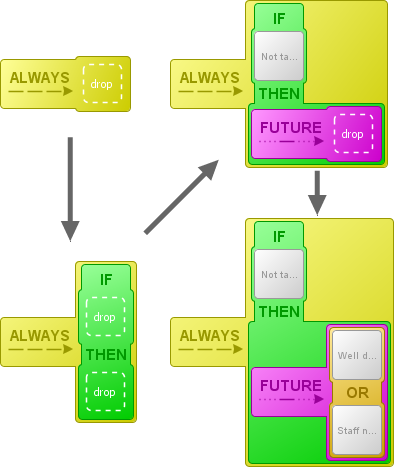
\includegraphics[scale=0.65]{sampleconstraint}
  \caption{Visual constraint creation for LTL formula ~\ref{eq:sampleconstraint}.}
  \label{fig:sampleconstraint}
\end{figure}

After each change on the dashboard, the constraint is automatically recompiled and revalidated by using the underlying model checker. For syntactically invalid constraints, an ``incomplete'' sign is displayed in the respective tab. Otherwise, an animated ring indicates that validation is in pro\-gress and will finally result in either a ``valid'' or ``invalid'' sign.



\subsection{Usability}

Due to the optimized performance of NuSMV, even the validation of constraints on huge and complex programs is fast and allows rapid feedback. In addition, the validation itself runs in the background without locking the dashboard. Therefore waiting times and disruptions during constraint development can be avoided, which would likely be the case with conventional model checking where constraint development and constraint validation are alternating processes. Thus the \emph{LTLCreator} tool is considered an improvement for the developer experience.

It could be observed that the different color flavours of the visual operators are a good support for fast reading and understanding of constraints. Also the two dimensional composition and the round shapes of the operators turned out to give the language a schematic but not too rectangular look. Besides it is considered eye-candy what is the best motivation for using this visual language.





\subsection{Expressiveness}

Due to being based on LTL, the visual language's expressivenes is equivalent to LTL's one of course. More precisely, that means any temporal logic formula can be expresssed except potentiality.
Furthermore there is one more limitation in the current visual language concerning the variety of available proposition operators. The visual language was originally designed for validating healthcare applications where just one kind of proposition is needed: ``currently state x is active''. Thus other propositions such as equations, comparisons with greater than etc.\ are not implemented yet, but can be easily integrated.
Figure~\ref{fig:example_propositions} depicts how an extension of \emph{LTLCreator} with additional proposition operators could be realized.

\begin{figure}[htbp]
  \centering
  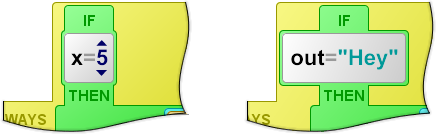
\includegraphics[scale=0.65]{example_propositions}
  \caption{Possible proposition extensions: Numeric and string equations.}
  \label{fig:example_propositions}
\end{figure}



\section{Automated constraint generation}
\label{sec:testscenarioandevaluation_automatedconstraintgeneration}

The automated constraint generation can be triggered by a click on the magic wand button in the tab area. After activation a dashboard is opened in a new tab for each constraint found, and validation is initiated immediately. For the medication reminder application six constraints are found, including \emph{a)} and \emph{b)} shown in figure~\ref{fig:generatedconstraints} which match the postulations in the requirements in chapter~\ref{chap:goals}.
The constraint used for demonstration in the previous section is also generated, however \emph{b)} forms an intensified restriction of it.
Constraint \emph{a)} ensures the ``Polling'' state is always eventually visited again. If a pending medication is not already taken, constraint \emph{b)} guarantees intake or staff notification before the next reminders can be read from the database.
Two more constraints are found which might be quite interesting for other programs; however, they do not contribute to safe behaviour of the medication reminder example and are less relevant.
The search and generation process finishes within less than a second and thus does not let developers wait for a long time.

It was showed that the subgraph approach is working for the medication reminder application, and there was even one more reasonable constraint found by the heuristic: Constraint \emph{c)} ensures that during the medication intake process the program can not switch back to the menu or other services such as entertainment or blood pressure measurement.



\begin{figure}[htbp]
  \centering
  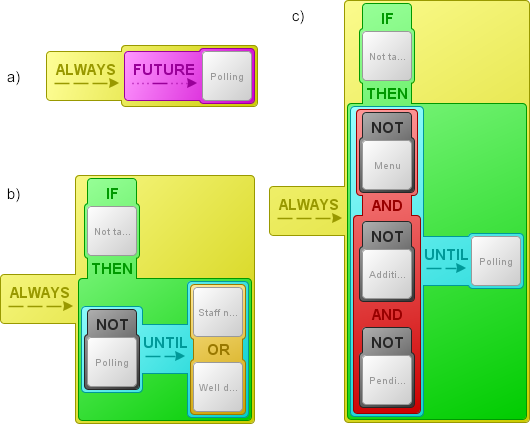
\includegraphics[scale=0.65]{generatedconstraints}
  \caption{Automatically generated constraints which match the required pos\-tu\-la\-tions.}
  \label{fig:generatedconstraints}
\end{figure}






\subsection{Performance}
\label{sec:performance}

In order to examine the performance of subgraph finding and constraint generation, the implementation details of the algorithm have to be analyzed. The subgraph finding algorithm is realized similar to a depth-first search. Indeed all healthcare programs are infinite and contain cycles and a depth-first walk-through would never end, but as stated in section~\ref{sec:prototype:automatedconstraintgeneration} the algorithm does not revisit already visited states.

The performance of this algorithm of course highly depends on the grade of branching. In contrast to a usual depth-first search in trees, the modified depth-first search is applicable for even cyclic state machines and will walk through all possible paths starting from one particular start state but without visiting states twice. Being $S$ the set of all states and $|S|$ the number of all states, and assuming the worst case in which every state has transitions to all other states, each of the remaining $|S|-1$ states can be possibly visited next, similarly $|S|-2$ for the third step and so on. As a worst case execution time the following result is obtained:

%Nevertheless, such a depth-first search has a worst case execution time of $O(|V|+|E|)$ in which $|V|$ is the number of states and $|E|$ number of edges respective transitions in our case.
%Since we cope with state machines and thus have directed edges rather than undirected ones, each state can have $|V|$ transitions; $|V|-1$ to other ones and one to itself. For the contained tree without cycles for depth-first search we retreive $|E|=|V|$ edges.
%As worst case ececution time for the depth-first search we obtain the following result:

\begin{equation}
O(\textnormal{``depth-first search''})=O((|S|-1)*(|S|-2)*...*2*1)=O((|S|-1)!)
\end{equation}

In order to find a subgraph with the presented algorithm the depth-first search has to be startet on a start state of a subgraph. Since it is not known in beforehand which states might be possible candidates for such start states, the algorithm has to be applied on every single state of the program which has two ore more outgoing transitions. In the worst case all $|S|$ states fulfil this condition, so the depth-first search has to be executed $|S|$ times. This implies for the estimated worst case execution time:

\begin{equation}
O(\textnormal{``subgraph finding''})=O(|S|)*O((|S|-1)!)=O(|S|!)
\end{equation}



\subsection{Scalability}

For all the healthcare applications that were examined, the presented algorithm works efficient and fast. But their program sizes are still quite manageable. The test program has eleven states, an average branching grade of $1.\overline{63}$ outgoing transitions per state and a constraint finding execution time of a split second on a standard computer.
Of course an exponential or factorial execution time is bad if the number of states arises. A clear slowdown can therefore be felt if the algorithm runs on larger state machines with plenty of states and a high grade of branching. A test on a state machine with over 250 states and partially high branching grade resulted in approximately five minutes execution time.

However, this algorithm for subgraph finding is not sophisticated regarding efficiency. It is rather a prototype to show the concept of automated constraint generation working and to provide this feature in the editor for evaluation. In case that this algorithm shall be used for other huge programs regardless its tailoring to the healthcare domain, the author is convinced that a more efficient algorithm for subgraph finding might be found by researchers.

%it keeps a lot of potential to be improved in efficiency. With a sophisticated approach it might be enough to execute just one depth-first search for finding all subgraphs at once what would lead to a linear execution time.
% wenn noch schreiben will, dann: linear ist cool, weil das tool eh die gefundenen constraints gleich anzeigt und nicht erst am ende alles geballt bringt.





\subsection{Reasonability of generated constraints}

The constraint generator algorithm found six constraints for the medication reminder application. Two of them were actually the ones proposed in the requirements. Three of them are either intensified versions of the proposed ones or just describe the behaviour of the program and therefore make sense, but in matters of safety they are not fundamental relevant.
Nevertheless the generator tool actually found a new important constraint which had not been considered before. It is constraint \emph{c)} in figure~\ref{fig:generatedconstraints} of section~\ref{sec:testscenarioandevaluation_automatedconstraintgeneration}.

To put it in a nutshell, in context of this example all automatically generated constraints are practical, and approximately half of them are significant. This shows that the constraint generator concept works well for the healthcare application and can be a very helpful feature.




\section{Practical experiences}
\label{sec:practicalexperiences}

Some parts of the healthcare robot's behaviour are appropriate to be specified by non-programmers, and that is the purpose of the presented visual language as well. Different tools and environments, among Robostudio and \emph{LTLCreator}, try to provide a particular interface suitable for such people. Now, it might be interesting to find out about user's experiences and how they get along when using these tools.

The \emph{LTLCreator} has been presented to several people, technical engineers as well as ordinary persons. The overall feedback was good and the idea and realization of the visual language was well-received. One of the laypersons who have been introduced to \emph{LTLCreator} was Alina Kracker. The 21 yeras old German student of educational science is also working for the elderly in a care facility since more than five years. In this social institution Ms. Kracker takes care of persons having different disease patterns and necessities. This spectrum varies from physical disabilities over mental problems such as Alzheimer's desease to being bedridden.
Her professional care background makes her feedback about usability and comprehensibility of the visual concept especially interesting since its application and testing was done in the healthcare domain.

Ms. Kracker was introduced to the example of medication reminder, and the program behaviour was described with the help of figure~\ref{fig:medicationreminder}. Afterwards she got familiarized with surface and functionality of \emph{LTLCreator}. Now, she was asked to formulate the two constraints postulated in the requirements, just by using the available means of the editor placed at her disposal.
The first constraint, which ensures the state ``Polling'' always eventually to be visited again, was constructed quickly and accurately by her.
The second constraint specifies, that every visit of state ``Not taken yet'' will eventually result in a visit of either state ``Well done!'' or ``Staff notified''. It turned out that this constraint held some difficulties for her: The \emph{FUTURE} operator was not considered initially by her. But it was also finished after a few consideration breaks.

Ms. Kracker did not know in beforehand what state machines are and never came in contact with LTL or model checking in general. But she dealt with this example and the visual language surprisingly well, and she is convinced that she could use it after some exercise. As reason for the success she pointed out the easy readability of the visual language and its close relationship to spoken language. Furthermore the intuitive drag and drop allowed fast editing.
Her examination on the visual language gives the evidence of success with the approach of creating an easy to use concept for defining LTL formulas. The visual language developed in this work enables even non-professionals to use the usually quite complex concept of model checking.

To the question, whether she would recommend such robotic services like the medication reminder application for use in the care facility she is working in, Ms. Kracker replied: ``I can envision such robot applications beeing an excellent assistance for the elderly who are mentally fit but maybe a little doolally. However, in our facilities most of the patients are not capable enough anymore of making decisions based on what the robots ask. In fact, due to frequent changes of the patients in our facilities it is a big issue for us care givers not to forget time-dependend medication intakes of our patients. Thus, such a reminding robot application would constitute an excellent support for us staff!''.
\chapter{Conclusion \& future work}
\label{chap:conclusionandfuturework}

%first step towards safety certification

This work presented a visual formalism for the defining of safety constraints and first steps towards a concept of automatic constraint generation. Both features are implemented and assembled in an editor for standalone or integrated use. The visual language is reasonably simple which makes it accessible to a wider range of software developers. Nevertheless it is reasonably expressive and allows serious model checking.

The concept of applying hueristics for proposing possible constraints to users of the visual language produced very good results in the healthcare use case, the medication reminder application. All postulated constraints were found and even a new reasonable constraint was discovered. Thus we are convinced that this approach, as well as the visual language for defining constraints itself, has the potential to really support users in development of safety critical robot applications in the healthcare domain and also other domains.

Perhaps the most important next step we identified is the application of the language and the constraint generation heuristic to other domains and applications. This will reveal if the identified subgraph-based heuristic for constraint generation provides reasonable results also in different scenarios. Most likely, it will be necessary to identify further heuristics and integrate them in the visual language editor to improve user support. A study among a group of users from the healthcare robotics domain could indicate the potential of usability improvements.

Some improvements on the feature side of the language or the editor were already identified. For example, the state proposition (currently the only supported proposition type) used in constraint formulation might be not enough for other domains. Supporting propositions based on strings or numerical equations might be necessary.
For reasons of enhancing the visual language, a substitution operator could be provided. Already existing constraints could be reused as parts of more complex constraints and thus simplify the overall look.
Finally, the only result of constraint checking presented to the user currently is whether the constraint is valid or invalid. In contrast to conventional model checking no additional explanation for the outcome such as a counter example is given. It can be considered to extend the visual language with support for bug identification by a visualization of counter examples, for example.
%\item Substitution of parts of constraints would be nice in order to make it easier to understand. (A simple operator which abstracts from a more complex operator). It's comparable to composite states of hirachical state machines.

%\item A feature which can display an counter example in case a constraint is not valid. It would make the user comprehend the reason in what situation a constraint fails.

%	\item constraints bewerten (nach gewichtung?) und nur wichtige vorschlagen? Oder zumindest sortieren


%\begin{itemize}
%	\item Yet, there are only states and no variable expressions etc.
%	\item Substitution of parts of constraints would be nice in order to make it easier to understand. (A simple operator which abstracts from a more complex operator). It's comparable to composite states of hirachical state machines.
%	\item A feature which can display an counter example in case a constraint is not valid. It would make the user comprehend the reason in what situation a constraint fails.
%	\item Problem mit der Zustandsbenennung! Die Zust�nde m�ssen passende Namen haben, was aber nicht immer m�glich ist. Daher m�sste man eigentlich auch Transitionsbedingungen in den Constraints erlauben
%	\item constraints bewerten (nach gewichtung?) und nur wichtige vorschlagen? Oder zumindest sortieren
%	\item �bertragbarkeit auf andere dom�nen untersuchen?
%	\item A bigger generation algorithm. As already metioned our approach only targets the healthcare domain. Especially the constraint generation can be improved to match also other domains.
%\end{itemize}

%1. Save and load functionality of constraints
%2. Yet, there are only states and no variable expressions etc.
%3. Substitution of parts of constraints would be nice in order to make it easier to understand. (A simple operator which abstracts from a more complex operator). It's comparable to composite states of hirachical state machines.
%4. A feature which can display an counter example in case a constraint is not valid. It would make the user comprehend the reason in what situation a constraint fails.
%5. A bigger generation algorithm
%6. constraints bewerten und nur wichtige vorschlagen? Oder zumindest sortieren
%7. uebertragbarkeit auf andere domaenen untersuchen?

\chapter*{Acknowledgment}

%This work evolved from a master thesis project provided by the Elite Graduate Program Software Engineering. 
%For the received support I would like to thank the people of this program and the three patron universities: University of Augsburg, Technical University Munich and Ludwig-Maximilians-University Munich.

\nocite{principles-of-model-checking}

\bibliographystyle{unsrt}
\bibliography{Bib}

\end{document}